% Options for packages loaded elsewhere
\PassOptionsToPackage{unicode}{hyperref}
\PassOptionsToPackage{hyphens}{url}
\PassOptionsToPackage{dvipsnames,svgnames,x11names}{xcolor}
%
\documentclass[
  10,
  letterpaper,
  DIV=11,
  numbers=noendperiod]{scrartcl}

\usepackage{amsmath,amssymb}
\usepackage{iftex}
\ifPDFTeX
  \usepackage[T1]{fontenc}
  \usepackage[utf8]{inputenc}
  \usepackage{textcomp} % provide euro and other symbols
\else % if luatex or xetex
  \usepackage{unicode-math}
  \defaultfontfeatures{Scale=MatchLowercase}
  \defaultfontfeatures[\rmfamily]{Ligatures=TeX,Scale=1}
\fi
\usepackage{lmodern}
\ifPDFTeX\else  
    % xetex/luatex font selection
\fi
% Use upquote if available, for straight quotes in verbatim environments
\IfFileExists{upquote.sty}{\usepackage{upquote}}{}
\IfFileExists{microtype.sty}{% use microtype if available
  \usepackage[]{microtype}
  \UseMicrotypeSet[protrusion]{basicmath} % disable protrusion for tt fonts
}{}
\makeatletter
\@ifundefined{KOMAClassName}{% if non-KOMA class
  \IfFileExists{parskip.sty}{%
    \usepackage{parskip}
  }{% else
    \setlength{\parindent}{0pt}
    \setlength{\parskip}{6pt plus 2pt minus 1pt}}
}{% if KOMA class
  \KOMAoptions{parskip=half}}
\makeatother
\usepackage{xcolor}
\setlength{\emergencystretch}{3em} % prevent overfull lines
\setcounter{secnumdepth}{-\maxdimen} % remove section numbering
% Make \paragraph and \subparagraph free-standing
\ifx\paragraph\undefined\else
  \let\oldparagraph\paragraph
  \renewcommand{\paragraph}[1]{\oldparagraph{#1}\mbox{}}
\fi
\ifx\subparagraph\undefined\else
  \let\oldsubparagraph\subparagraph
  \renewcommand{\subparagraph}[1]{\oldsubparagraph{#1}\mbox{}}
\fi


\providecommand{\tightlist}{%
  \setlength{\itemsep}{0pt}\setlength{\parskip}{0pt}}\usepackage{longtable,booktabs,array}
\usepackage{calc} % for calculating minipage widths
% Correct order of tables after \paragraph or \subparagraph
\usepackage{etoolbox}
\makeatletter
\patchcmd\longtable{\par}{\if@noskipsec\mbox{}\fi\par}{}{}
\makeatother
% Allow footnotes in longtable head/foot
\IfFileExists{footnotehyper.sty}{\usepackage{footnotehyper}}{\usepackage{footnote}}
\makesavenoteenv{longtable}
\usepackage{graphicx}
\makeatletter
\def\maxwidth{\ifdim\Gin@nat@width>\linewidth\linewidth\else\Gin@nat@width\fi}
\def\maxheight{\ifdim\Gin@nat@height>\textheight\textheight\else\Gin@nat@height\fi}
\makeatother
% Scale images if necessary, so that they will not overflow the page
% margins by default, and it is still possible to overwrite the defaults
% using explicit options in \includegraphics[width, height, ...]{}
\setkeys{Gin}{width=\maxwidth,height=\maxheight,keepaspectratio}
% Set default figure placement to htbp
\makeatletter
\def\fps@figure{htbp}
\makeatother

\usepackage{booktabs}
\usepackage{longtable}
\usepackage{array}
\usepackage{multirow}
\usepackage{wrapfig}
\usepackage{float}
\usepackage{colortbl}
\usepackage{pdflscape}
\usepackage{tabu}
\usepackage{threeparttable}
\usepackage{threeparttablex}
\usepackage[normalem]{ulem}
\usepackage{makecell}
\usepackage{xcolor}
\usepackage{booktabs}
\usepackage{siunitx}
\newcolumntype{d}{S[
  input-open-uncertainty=,
  input-close-uncertainty=,
  parse-numbers = false,
  table-align-text-pre=false,
  table-align-text-post=false
]}
\KOMAoption{captions}{tableheading}
\makeatletter
\makeatother
\makeatletter
\makeatother
\makeatletter
\@ifpackageloaded{caption}{}{\usepackage{caption}}
\AtBeginDocument{%
\ifdefined\contentsname
  \renewcommand*\contentsname{Table of contents}
\else
  \newcommand\contentsname{Table of contents}
\fi
\ifdefined\listfigurename
  \renewcommand*\listfigurename{List of Figures}
\else
  \newcommand\listfigurename{List of Figures}
\fi
\ifdefined\listtablename
  \renewcommand*\listtablename{List of Tables}
\else
  \newcommand\listtablename{List of Tables}
\fi
\ifdefined\figurename
  \renewcommand*\figurename{Figure}
\else
  \newcommand\figurename{Figure}
\fi
\ifdefined\tablename
  \renewcommand*\tablename{Table}
\else
  \newcommand\tablename{Table}
\fi
}
\@ifpackageloaded{float}{}{\usepackage{float}}
\floatstyle{ruled}
\@ifundefined{c@chapter}{\newfloat{codelisting}{h}{lop}}{\newfloat{codelisting}{h}{lop}[chapter]}
\floatname{codelisting}{Listing}
\newcommand*\listoflistings{\listof{codelisting}{List of Listings}}
\makeatother
\makeatletter
\@ifpackageloaded{caption}{}{\usepackage{caption}}
\@ifpackageloaded{subcaption}{}{\usepackage{subcaption}}
\makeatother
\makeatletter
\@ifpackageloaded{tcolorbox}{}{\usepackage[skins,breakable]{tcolorbox}}
\makeatother
\makeatletter
\@ifundefined{shadecolor}{\definecolor{shadecolor}{rgb}{.97, .97, .97}}
\makeatother
\makeatletter
\makeatother
\makeatletter
\makeatother
\ifLuaTeX
  \usepackage{selnolig}  % disable illegal ligatures
\fi
\usepackage[]{natbib}
\bibliographystyle{plainnat}
\IfFileExists{bookmark.sty}{\usepackage{bookmark}}{\usepackage{hyperref}}
\IfFileExists{xurl.sty}{\usepackage{xurl}}{} % add URL line breaks if available
\urlstyle{same} % disable monospaced font for URLs
\hypersetup{
  pdftitle={Supplementary Appendix for Outside Threats and Public Perceptions of the U.S. Military in Poland},
  colorlinks=true,
  linkcolor={blue},
  filecolor={Maroon},
  citecolor={Blue},
  urlcolor={Blue},
  pdfcreator={LaTeX via pandoc}}

\title{Supplementary Appendix for Outside Threats and Public Perceptions
of the U.S. Military in Poland}
\author{}
\date{}

\begin{document}
\maketitle
\ifdefined\Shaded\renewenvironment{Shaded}{\begin{tcolorbox}[frame hidden, boxrule=0pt, borderline west={3pt}{0pt}{shadecolor}, sharp corners, breakable, interior hidden, enhanced]}{\end{tcolorbox}}\fi

\renewcommand*\contentsname{Table of contents}
{
\hypersetup{linkcolor=}
\setcounter{tocdepth}{3}
\tableofcontents
}
\hypertarget{overview}{%
\section{Overview}\label{overview}}

These appendices contain supplementary information for the paper
Supplementary Appendix for Outside Threats and Public Perceptions of the
U.S. Military in Poland. Herein we provide a number of additional
resources related to the project. First, we provide basic information
about the survey and data collection procedures. Second, we provide some
basic descriptive statistics and information to help readers better
understand the data and the distribution of key variables and responses.
Third, to save space in the primary manuscript we include all of the
model tables for the project here. Fourth, we also include a number of
additional figures to help communicate the results of our analysis.
Finally, we include a number of diagnostic plots generated from the
models we run. In general, we focus on a few specific types of plots
and, where necessary, on key variables. For example, traceplots for
multilevel multinomial logit models can quickly become both numerous and
unwieldy in the confines of a PDF or printed document.

\hypertarget{power-analysis}{%
\section{Power Analysis}\label{power-analysis}}

Before analyzing the data we developed a Bayesian power analysis in an
effort to evaluate the probability of correctly identifying true effects
versus false positives for the experimental treatment effects. We follow
\citet{kruschkeDoingBayesianData2015} in carrying out this test and
implement it in the following steps.

First, we wrote a function that would simulate data that look like the
expected sample data. In addition to our survey plan, we used data from
\citet{Allenetal2020} and \citet{Allenetal2022} to establish a baseline
expectation for what the distribution of the variables should look like.

Second, we generate a set of expected coefficient/effect values for all
of the variables in our model. Note that for each variable we allow the
expected effect to vary, establishing a mean and standard deviation for
the expected effect rather than fixing its value. Where our variables
overlap with those included in \citet{Allenetal2022}, we use their
posterior estimates to generate our expected effect sizes and
distributions. Where our variables differ (for example, we include
variables that capture respondents' income sources/occupational fields)
we set the expected effects to 0 with a standard deviation of 0.5 to
reflect our uncertainty in the parameter values. This does not apply to
the treatment variables, which we address more fully below. We also
include varying intercepts for the 16 Polish provinces to match our plan
to model the actual data using varying intercepts. In general, where we
expect an effect we set the standard deviation so it is less than half
of the mean beta value.

Third, following this procedure we generate 200 hypothetical data sets
for a given sample size value.

Fourth, we chose a set of hypothetical sample size values to evaluate
the model's ability to recover the expected parameter space.
Specifically, we choose sample sizes of 1600, 2560, 4800, and 12800. Our
actual data are close to 2500, but we chose the other values to assess
the model's performance across a wider range of hypothetical
circumstances.

In total, we end up with \(I \times K\) datasets and models, where \(I\)
is the number of iterations per sample size (i.e.~200) and \(K\) is the
number of different sample sizes (i.e.~4. In our case, we generate 800
sample data sets and run the model a total of 800 times. As in our
primary manuscript, we model the hypothetical data using a Bayesian
multilevel multinomial logistic regression using \texttt{\{brms\}}
\citep{Burkner2017, Burkner2018}.

For the treatment values, we do not have strong priors as to what
constitute accurate effects. Accordingly, we generate parameters with a
couple of considerations. First, given that we are estimating a
multinomial logistic regression, the plausible parameter space is fairly
constrained. Extreme values (e.g.~\(|\beta| > 4\)) are unlikely (except
in cases where observations appear to be rare). Second, we look at the
effect sizes on similar variables in \citet{Allenetal2020} and
\citet{Allenetal2022}. Third, we generally expect that the different
treatment prompts will increase support for a U.S. presence and decrease
opposition. However, we also expect they will yield different
magnitudes, with the combined treatment mentioning security concerns
\emph{and} economic benefits yielding the largest of the three. We also
view this as an opportunity to evaluate our ability to recover effects
of different sizes, and so we set the parameter distributions to values
that we think fall within the plausible range, but also run the range of
``small'' to ``large'' effects.

Given these considerations, the distributions we use in the power
analysis are as follows.

\begin{align}
\text{Support} &
\begin{cases}
Treatment_{SecurtyandEconomic} &\sim N(1.0, 0.3) \\
Treatment_{Security} &\sim N(0.5, 0.1) \\
Treatment_{Economic} &\sim N(0.1, 0.02) 
\end{cases} 
\\
\text{Oppose} &
\begin{cases}
Treatment_{SecurtyandEconomic} &\sim N(-0.8, 0.3) \\
Treatment_{Security} &\sim N(-0.5, 0.2) \\
Treatment_{Economic} &\sim N(-0.1, 0.05) 
\end{cases} 
\\
\text{Don't know/Decline to answer} &
\begin{cases}
Treatment_{SecurtyandEconomic} &\sim N(-0.5, 0.25) \\
Treatment_{Security} &\sim N(-0.2, 0.1) \\
Treatment_{Economic} &\sim N(-0.1, 0.08) 
\end{cases}
\end{align}

The following figures show the results of our power analysis. The first
figure shows the average \(Pr(Direction)\) score for the treatment
variables. The \(Pr(Direction)\) statistic tells us the proportion of
the posterior distribution that falls above/below 0 on the same side as
the median value. If we had a median coefficient estimate where the
median \(\beta = 0.5\) and \(Pr(Direction) = 0.97\), this tells us that
there is a 97\% chance of a positive effect. An average
\(Pr(Direction)\) of 0.90, for example, would therefore tell us that, on
average, there is a 90\% chance of a positive effect.

It is common to see power analyses presented in terms of what proportion
of models' 95\% confidence intervals exclude 0 and demonstrate an
effect. We adopt this alternative approach because it allows us to more
directly incorporate information about the posterior distribution into
our assessment than the conventional frequentist approach.

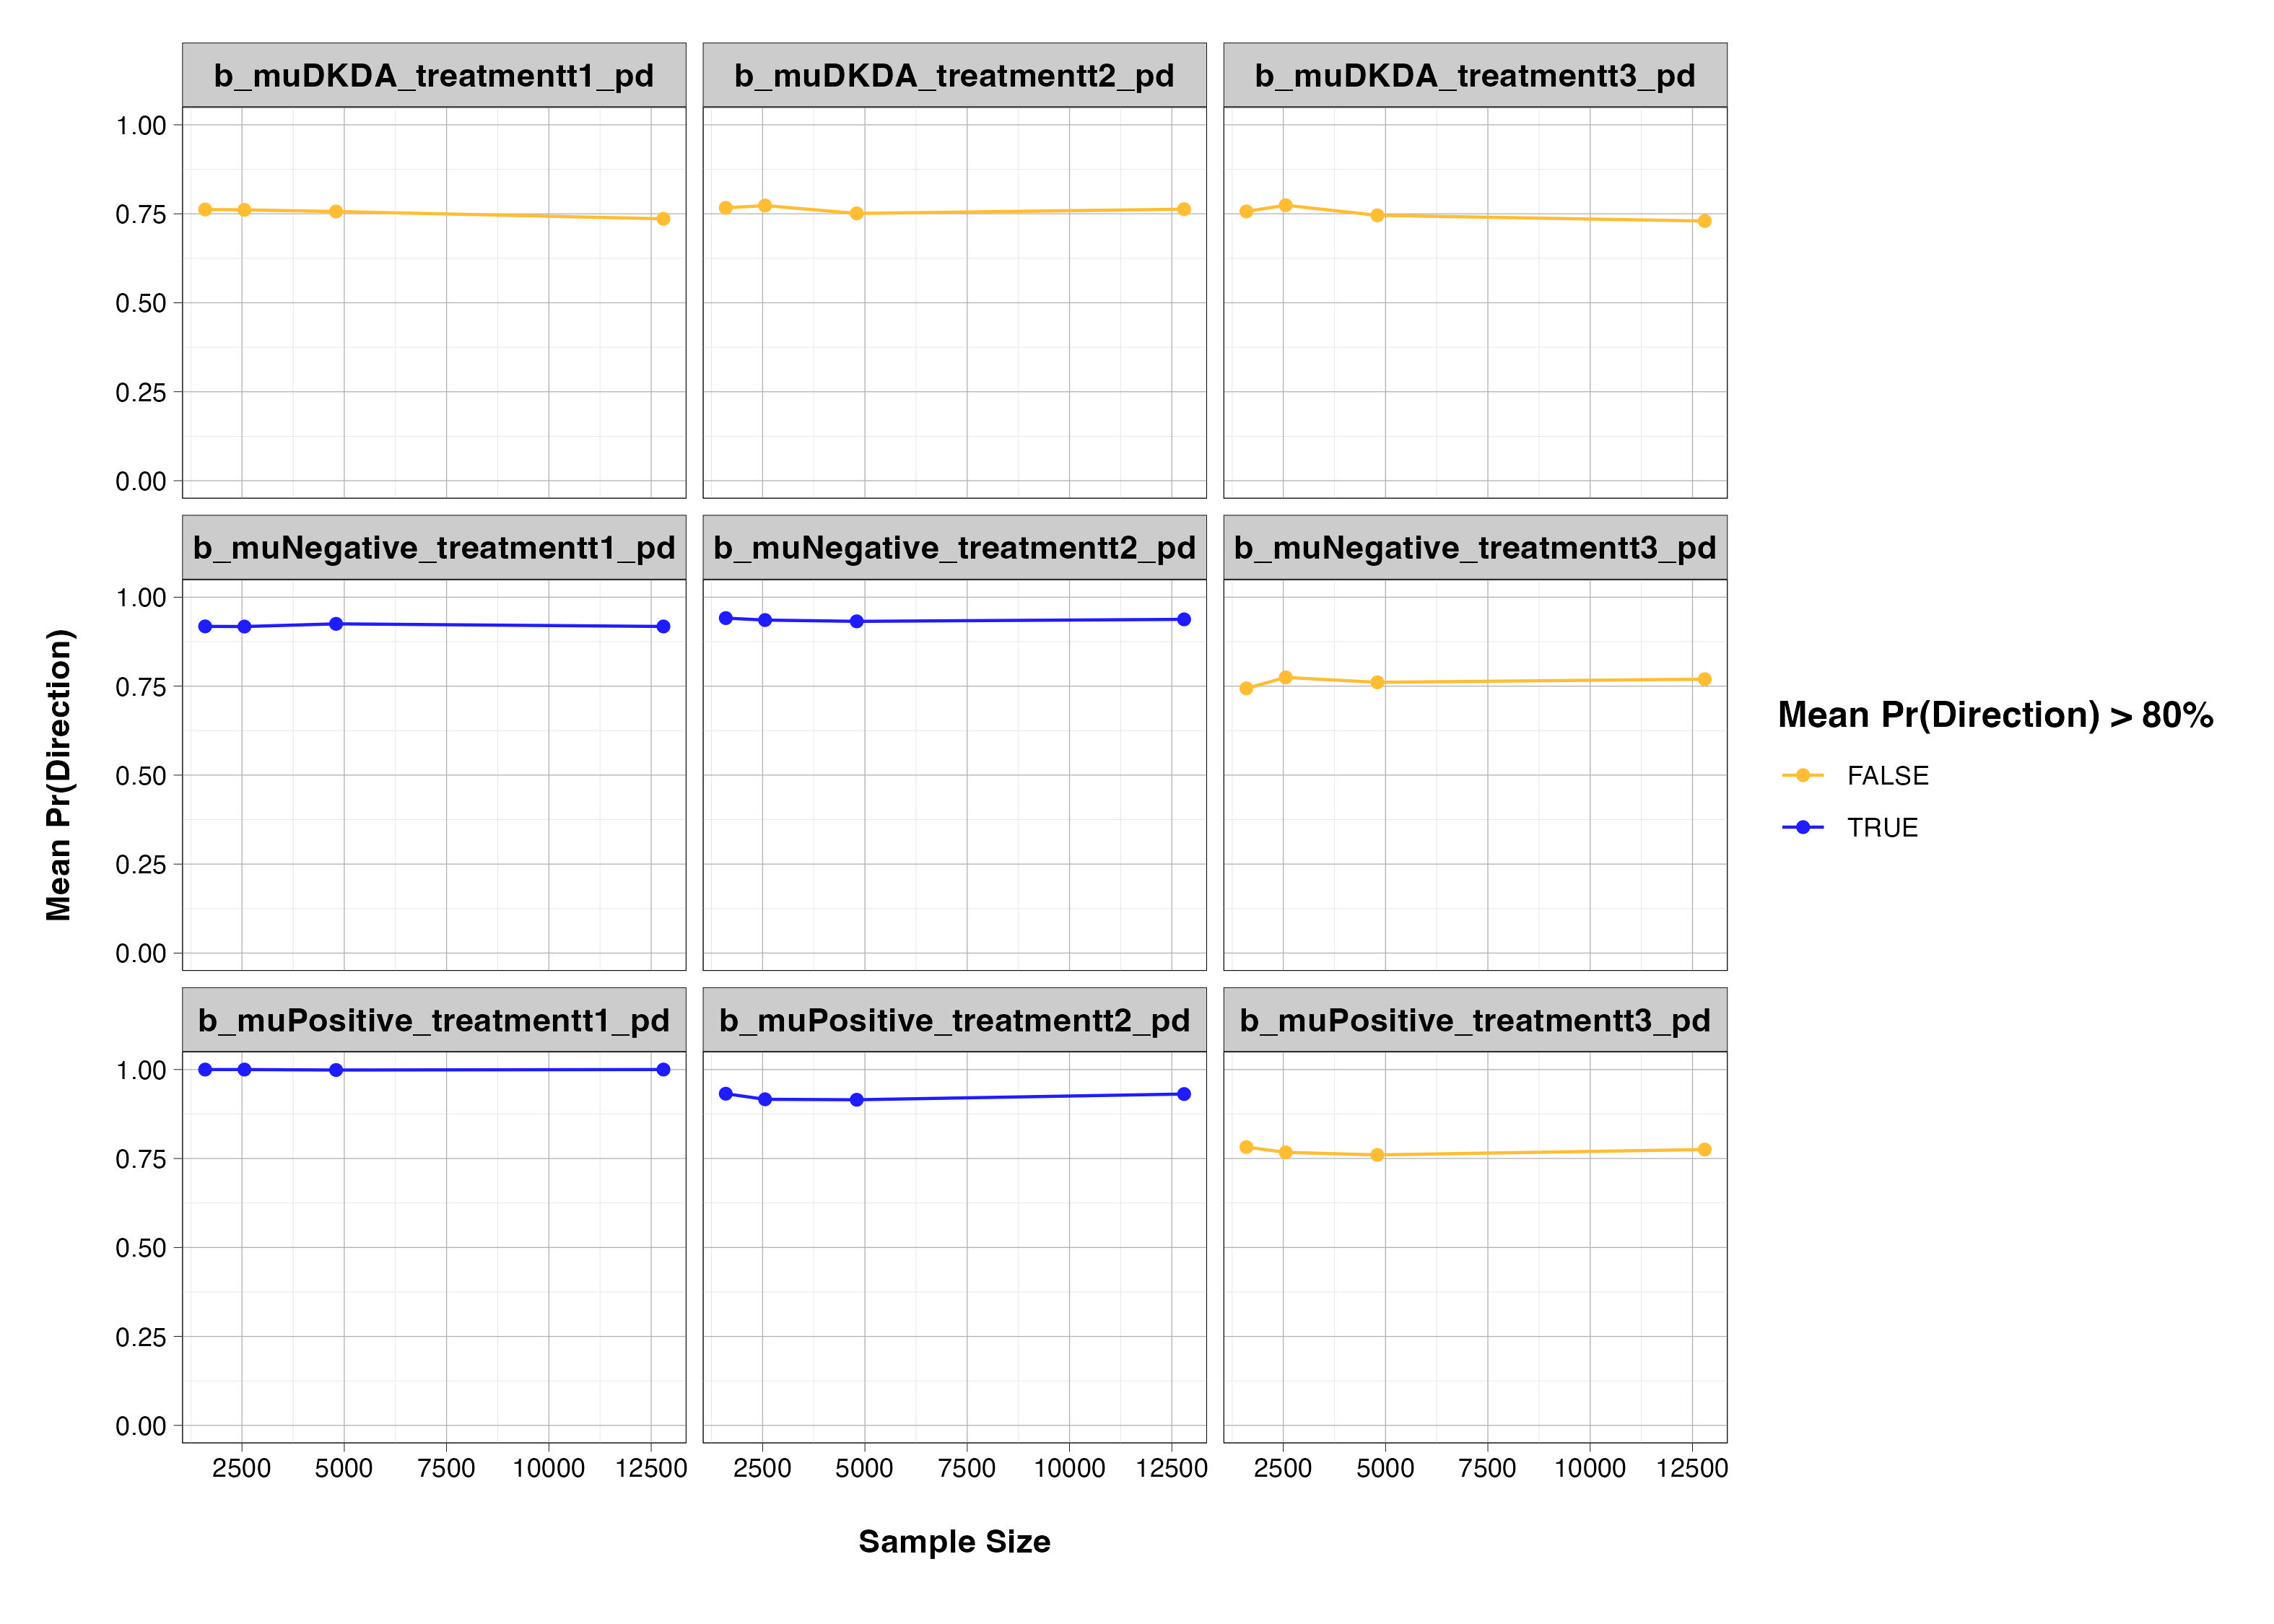
\includegraphics{../Figures/fig-sim-threshold.jpg}

The second figure shows spaghetti plots whereby the posterior
distributions for the treatment effects from the 200 different models
are overlaid on top of one another. While this figure does not provide
us with a specific statistic as in the case of the previous figure, it
does give us a visual check on the distribution of the recovered
coefficients and the accompanying uncertainty.

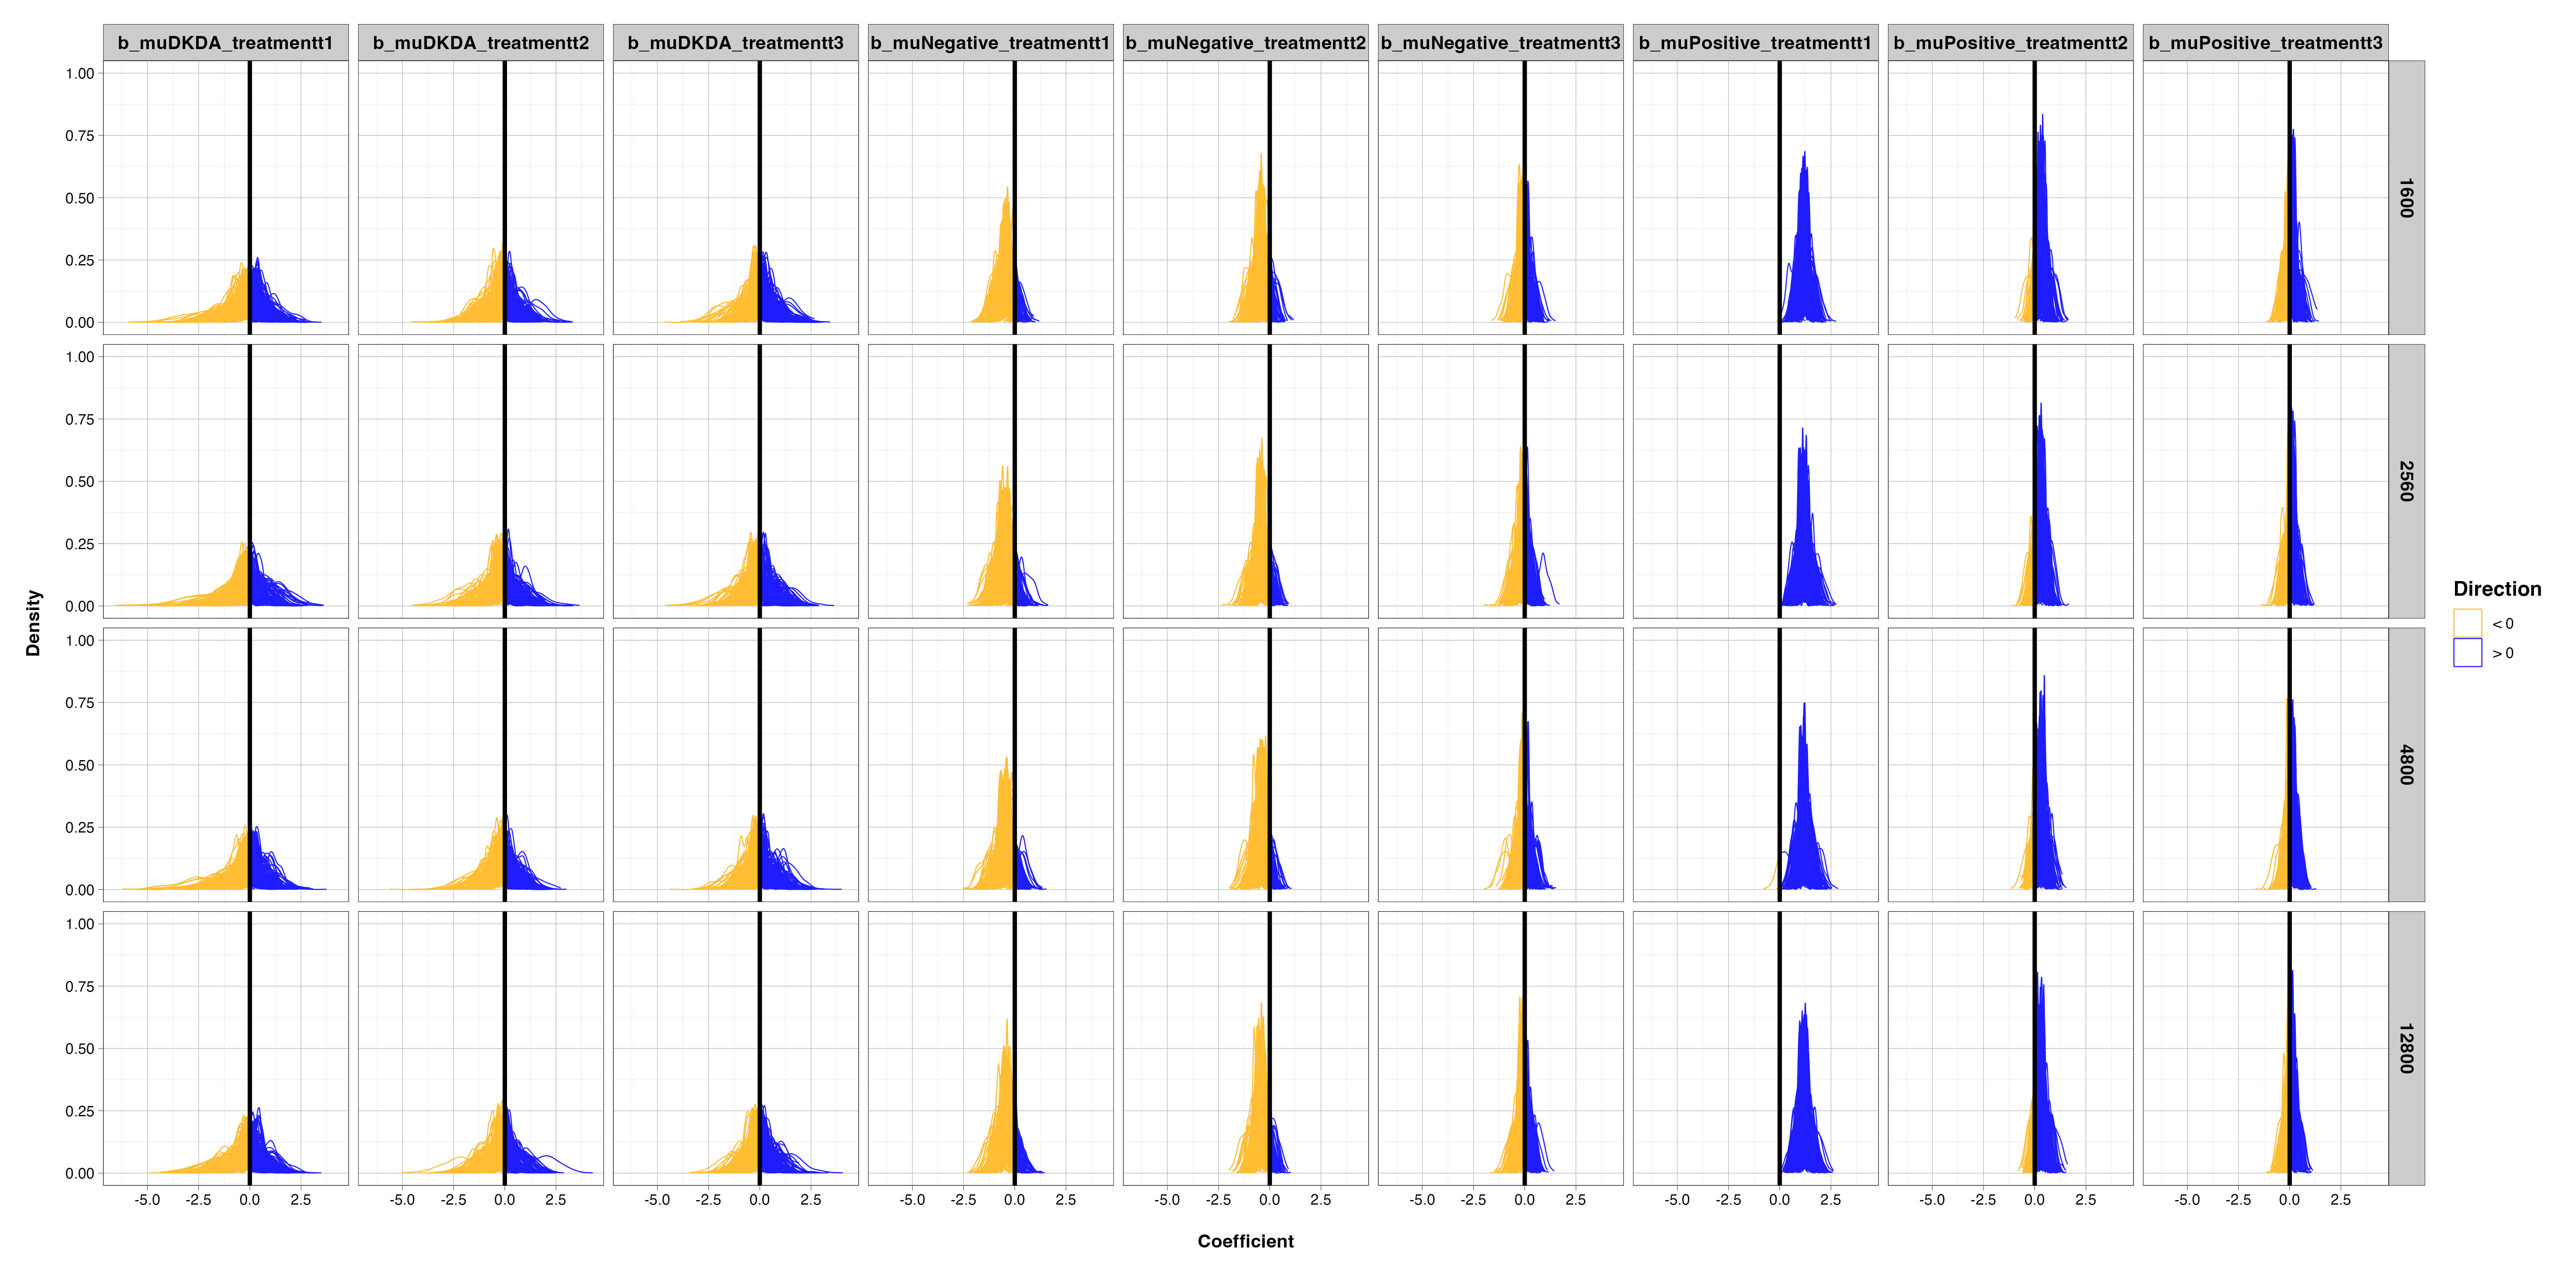
\includegraphics{../Figures/fig-sim-spaghetti.jpg}

In general, the models do a fairly good job of recovering the parameter
values we set in our simulation. The average \(Pr(Direction)\) score is
above 80\% for the first and second treatment variables in the Positive
and Negative response categories. The mean expected effect in these
cases is approximately 1.0, 0.5, and 0.1 f or the Positive response
equation and \(-0.8\), \(-0.5\), and \(-0.1\) for the negative response
model. For the Don't know/Decline response equation we set the expected
values to \(-0.5\), \(-0.2\), and \(-0.1\), but we set the standard
deviation to a higher value given the relatively low incidence of these
responses in existing data and the high level of uncertainty
accompanying these responses.

These results indicate that for the largest effect sizes we have a
fairly strong chance of recovering the parameter of interest. However,
for the smaller effect sizes we are looking at only a 70-75\% chance of
recovering the parameter of interest. Though this figure may seem high,
the smallest value that the \(Pr(Direction)\) statistic can take on is
(roughly speaking) 0.50 as it is necessarily tied to the median
posterior sample value. Since we do not set any of the Don't
know/Decline coefficients to values close to 0, it makes sense that the
posterior samples often have a ``larger'' portion of their distributions
falling below 0. Accordingly, we should be cautious in treating small
effects as definitive given our relatively small sample size.

However, our expectations regarding the effects of the treatments prove
to be quite wrong. As we discuss in the manuscript, and as we show in
the tables below, the treatment effects do not generally correlate
strongly with the outcome response. Overall, our expectations regarding
the effects of the informational prompts were wide of the mark.

\hypertarget{descriptive-figures}{%
\section{Descriptive Figures}\label{descriptive-figures}}

This section includes additional descriptive figures not included in the
primary manuscript.

\hypertarget{views-of-major-powers}{%
\subsection{Views of Major Powers}\label{views-of-major-powers}}

Figure~\ref{fig-views-us-troops} shows the distribution of views of U.S.
military personnel deployed to Poland in March of 2023 at the time of
our survey. This is a different representation of the 2023 data we show
in Figure 1 of the primary manuscript.

\begin{figure}

{\centering 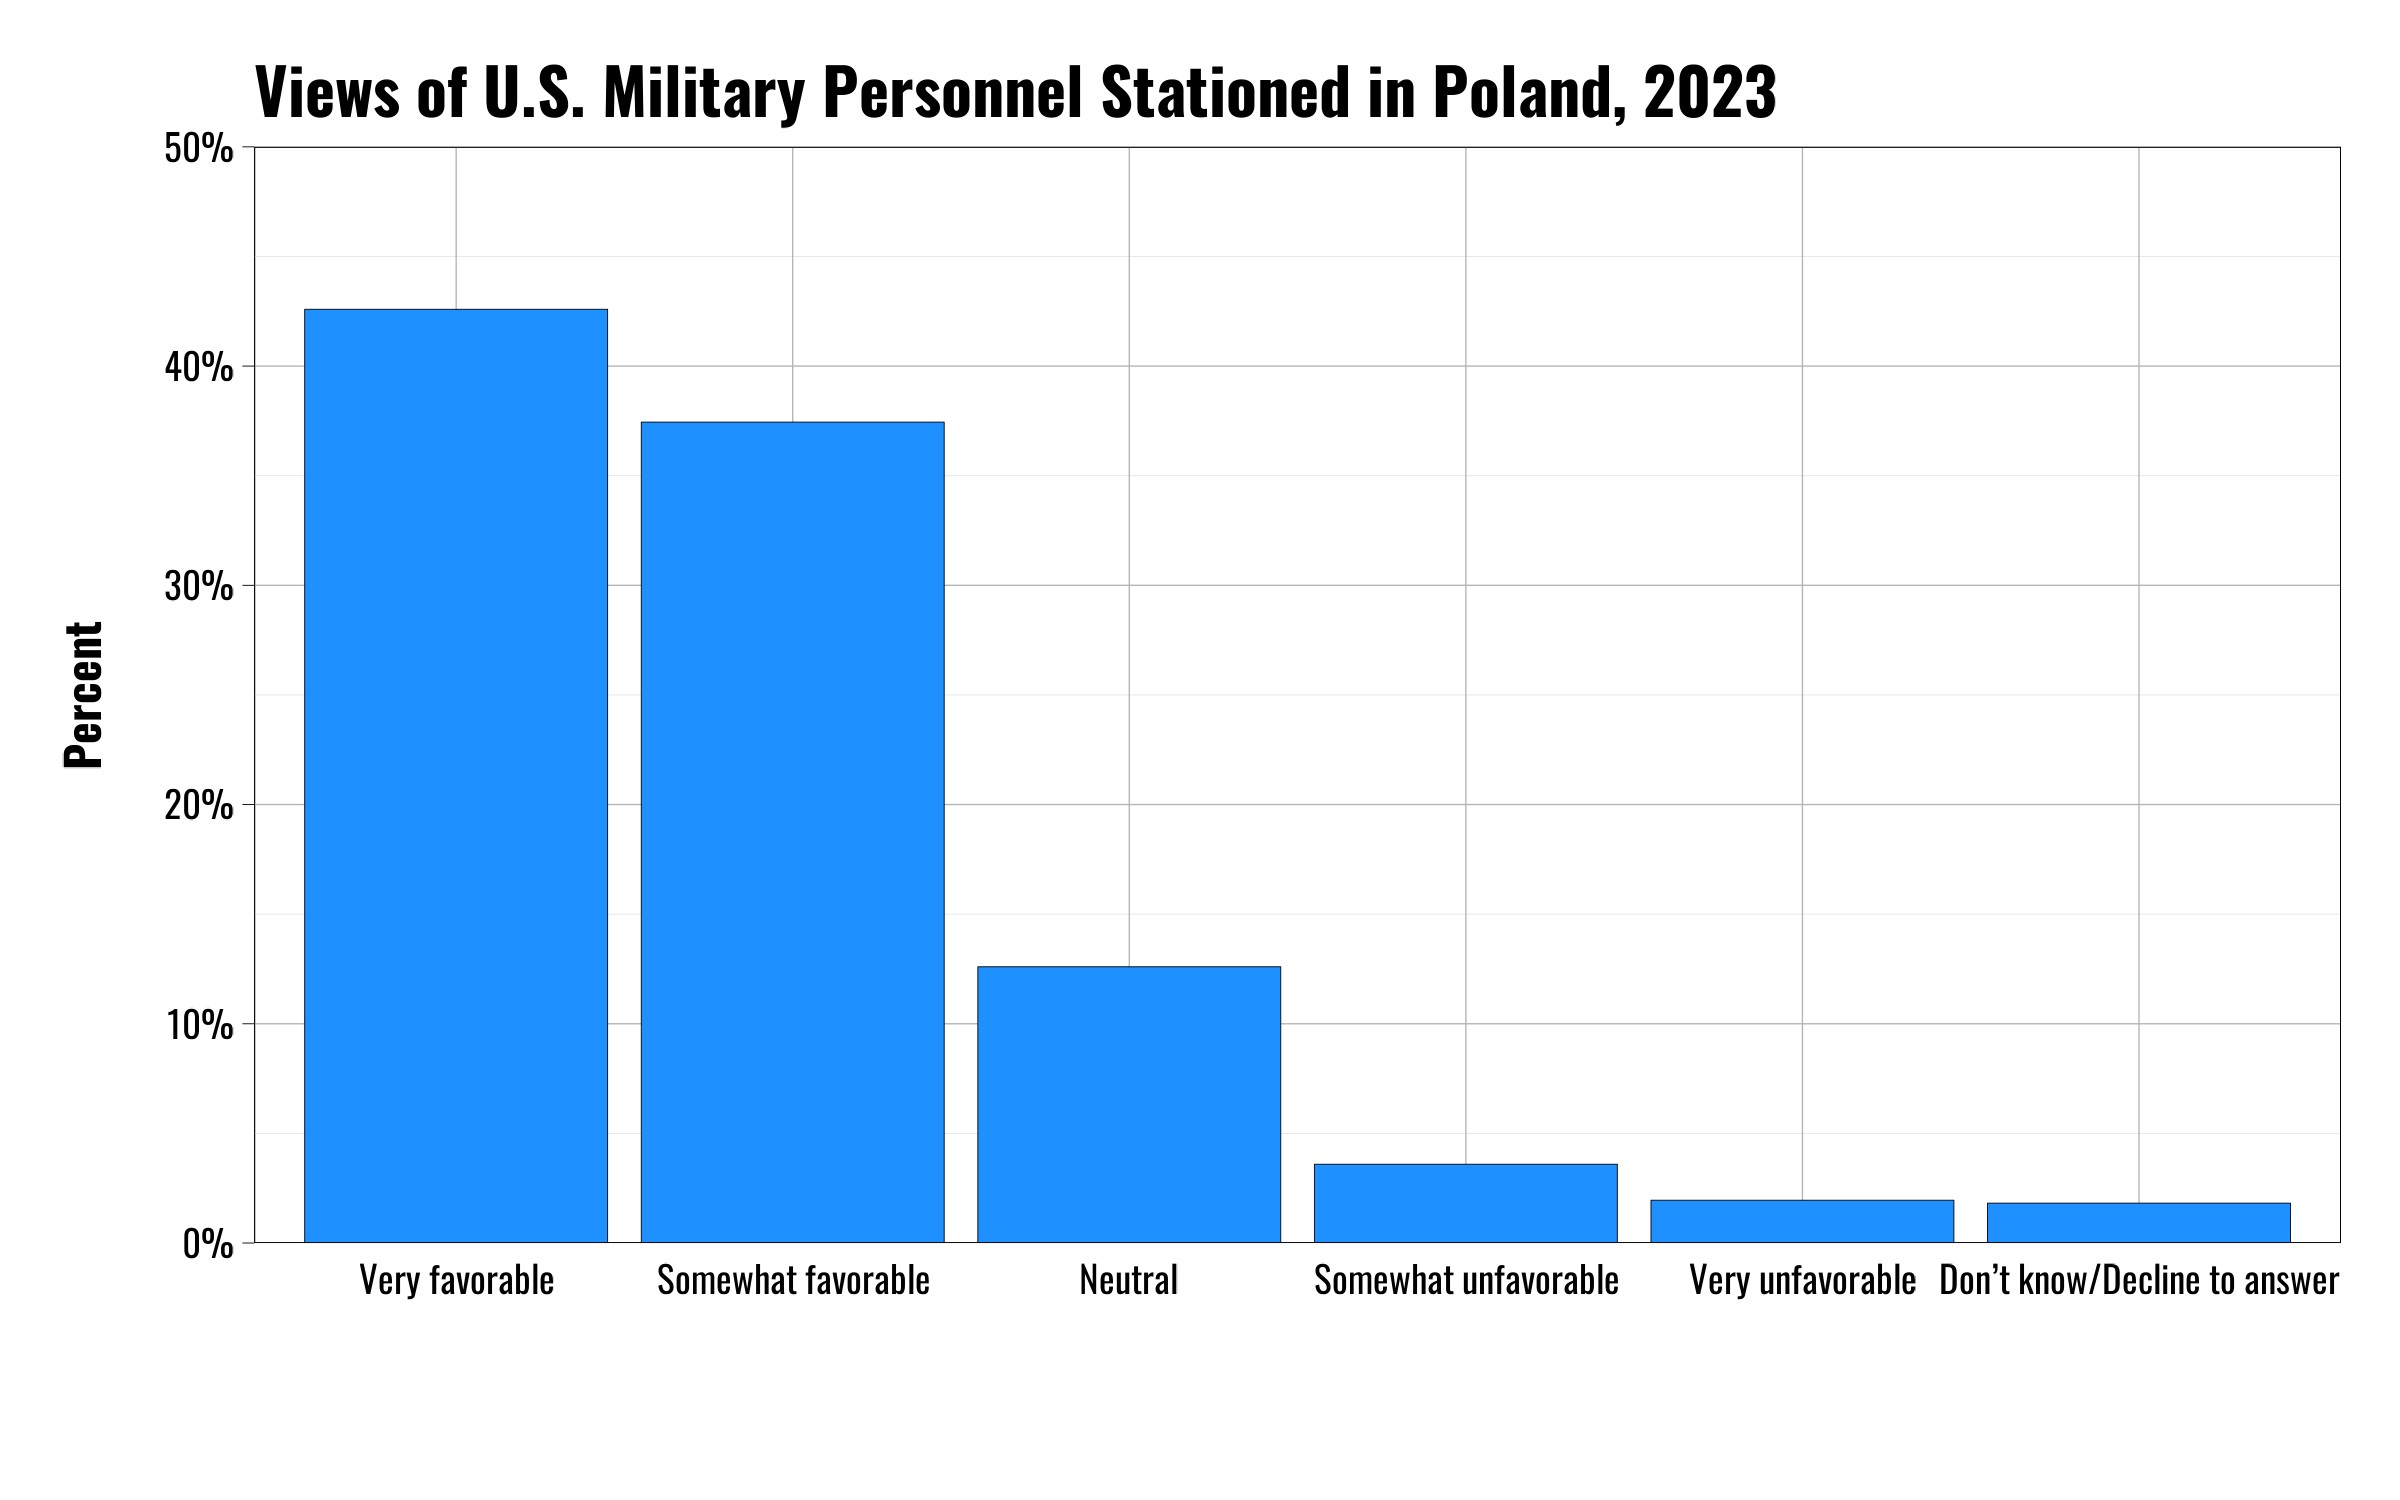
\includegraphics{../Figures/views-us-troops.png}

}

\caption{\label{fig-views-us-troops}Views of U.S. military personnel in
Poland among Polish adults}

\end{figure}

Figure~\ref{fig-views-russia} shows the distribution of Polish adults'
views of Poland's relations with Russia in March of 2023 at the time of
our survey.Overwhelmingly respondents indicate that relations between
Poland and Russia are ``Somewhat hostile'' or ``Very hostile.''

\begin{figure}

{\centering 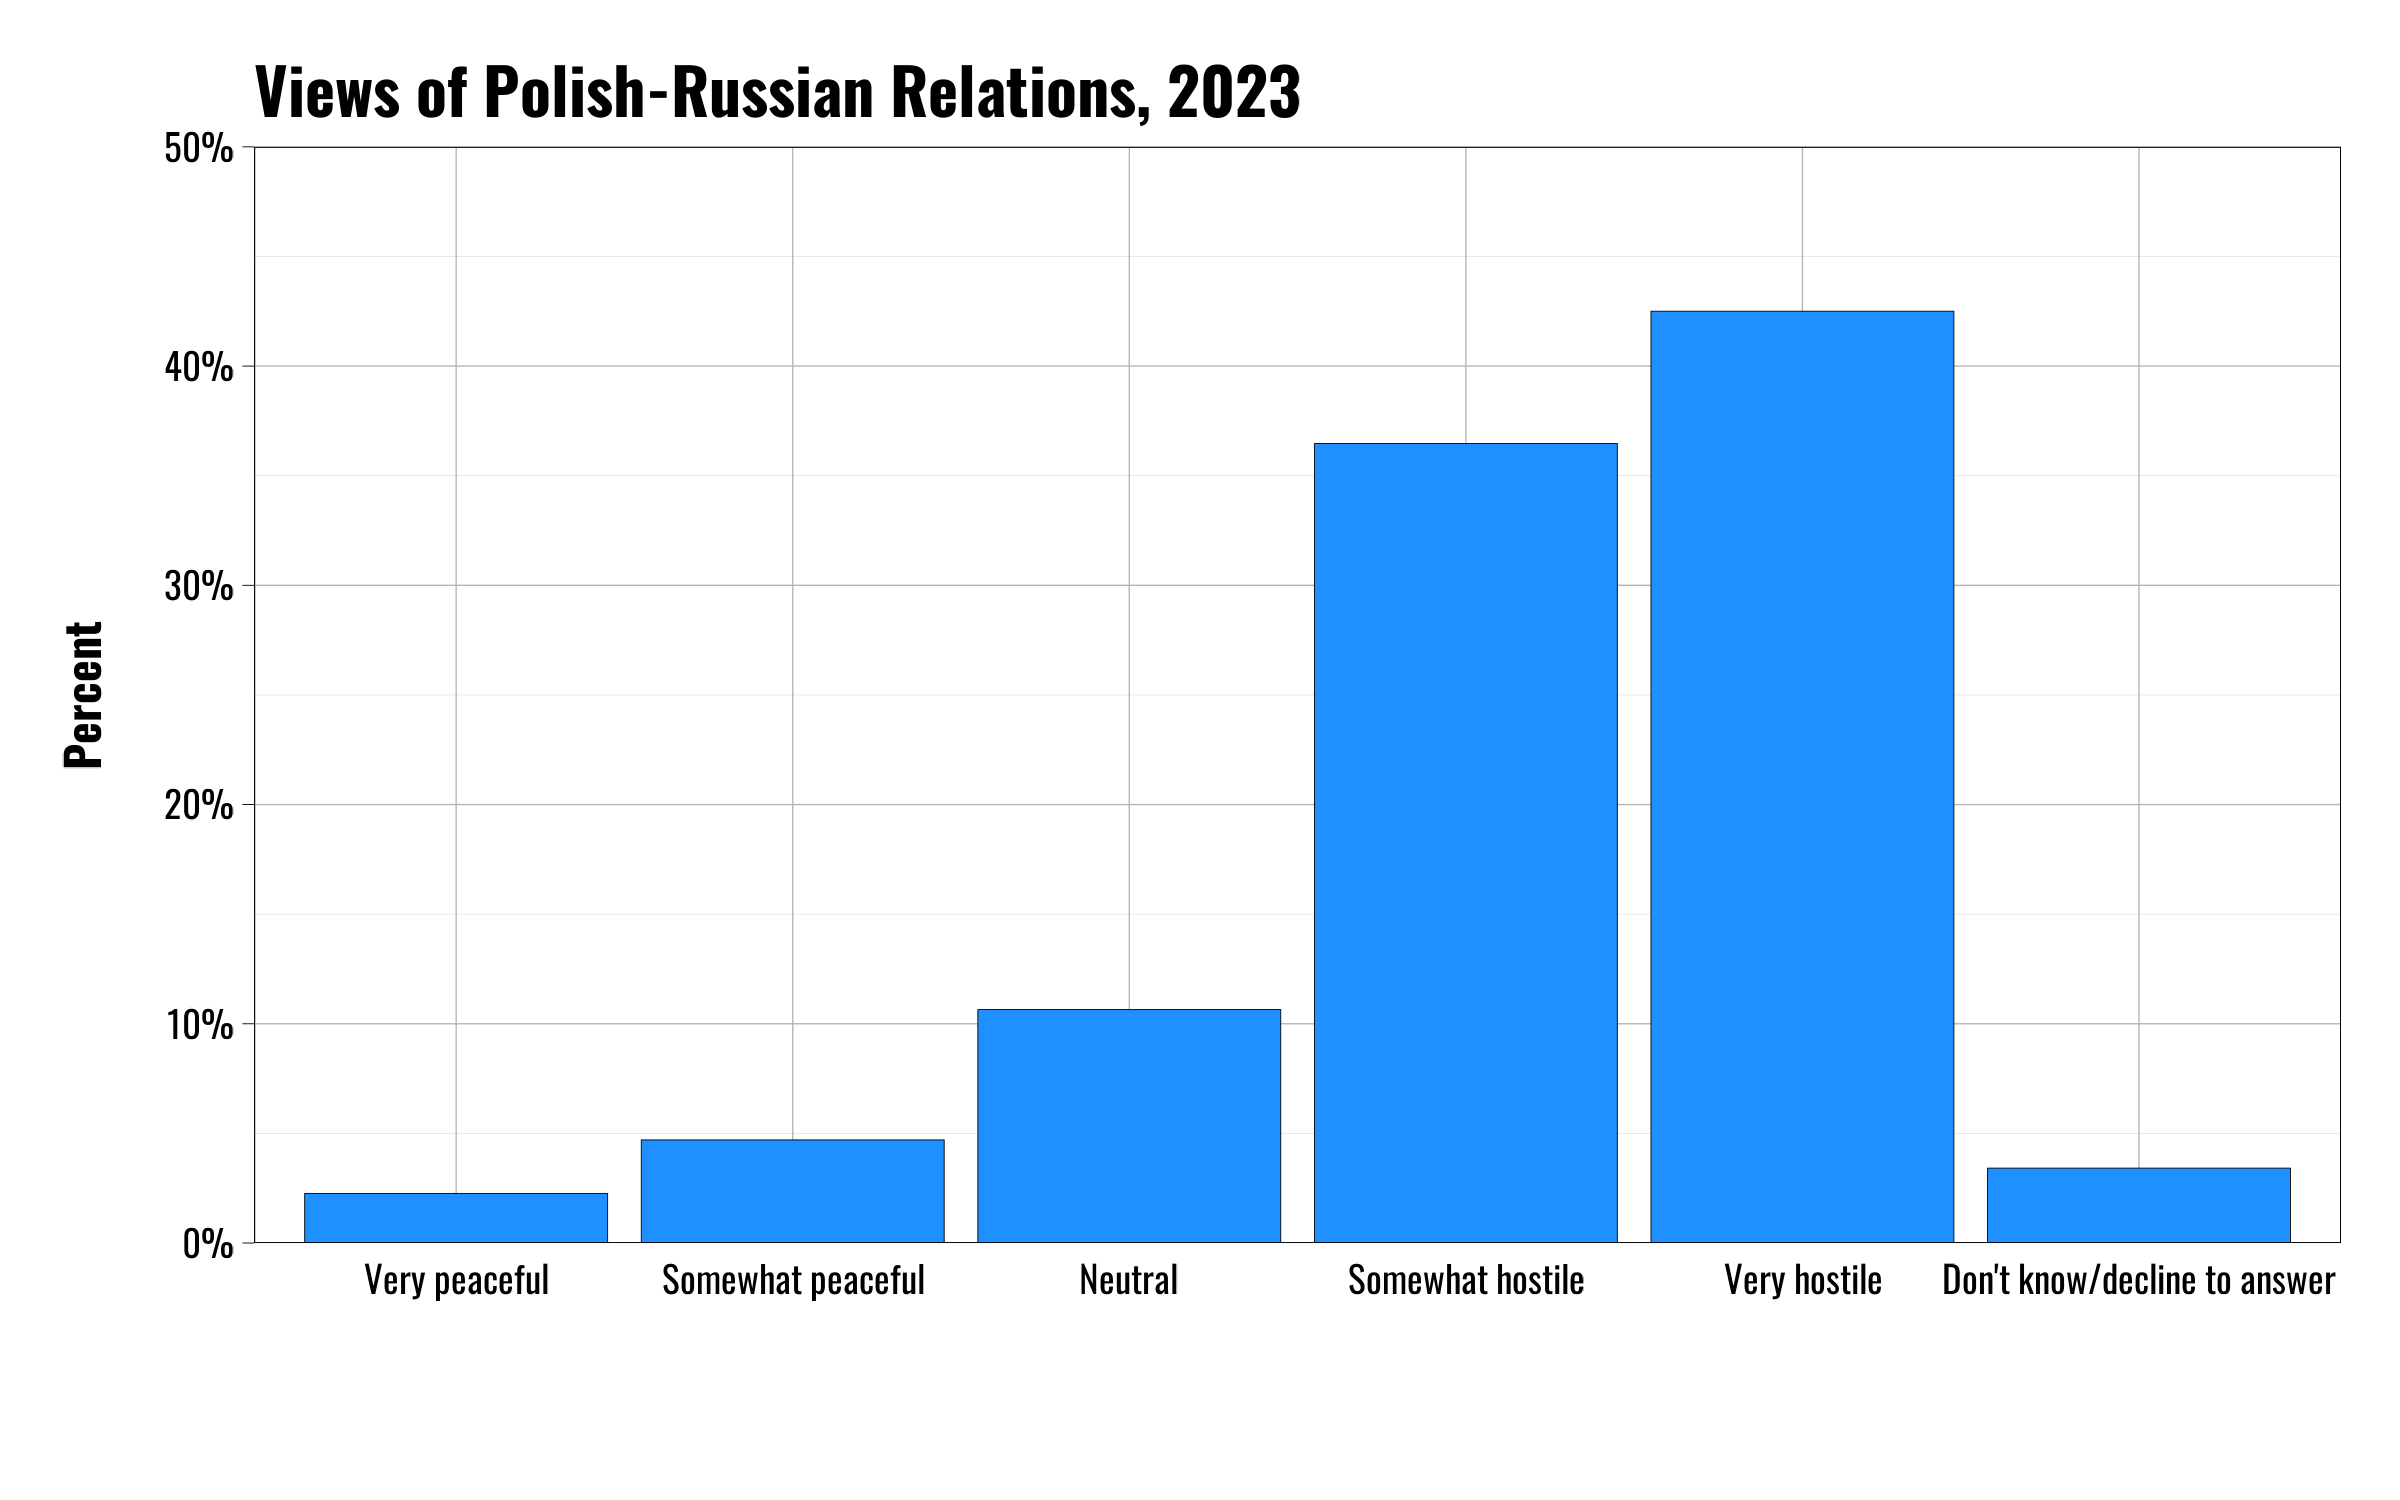
\includegraphics{../Figures/views-russian-relations.png}

}

\caption{\label{fig-views-russia}Views of Russia among Polish adults}

\end{figure}

\hypertarget{distribution-of-respondents}{%
\subsection{Distribution of
respondents}\label{distribution-of-respondents}}

Figure~\ref{fig-respondents-province} shows the number of respondents
per province In general, most of the group sizes fall between 100 and
200 respondents per province. The lowest number of respondents per group
is 52 (Opolskie) and the highest is 339 (Mazowieckie).

\begin{figure}

{\centering 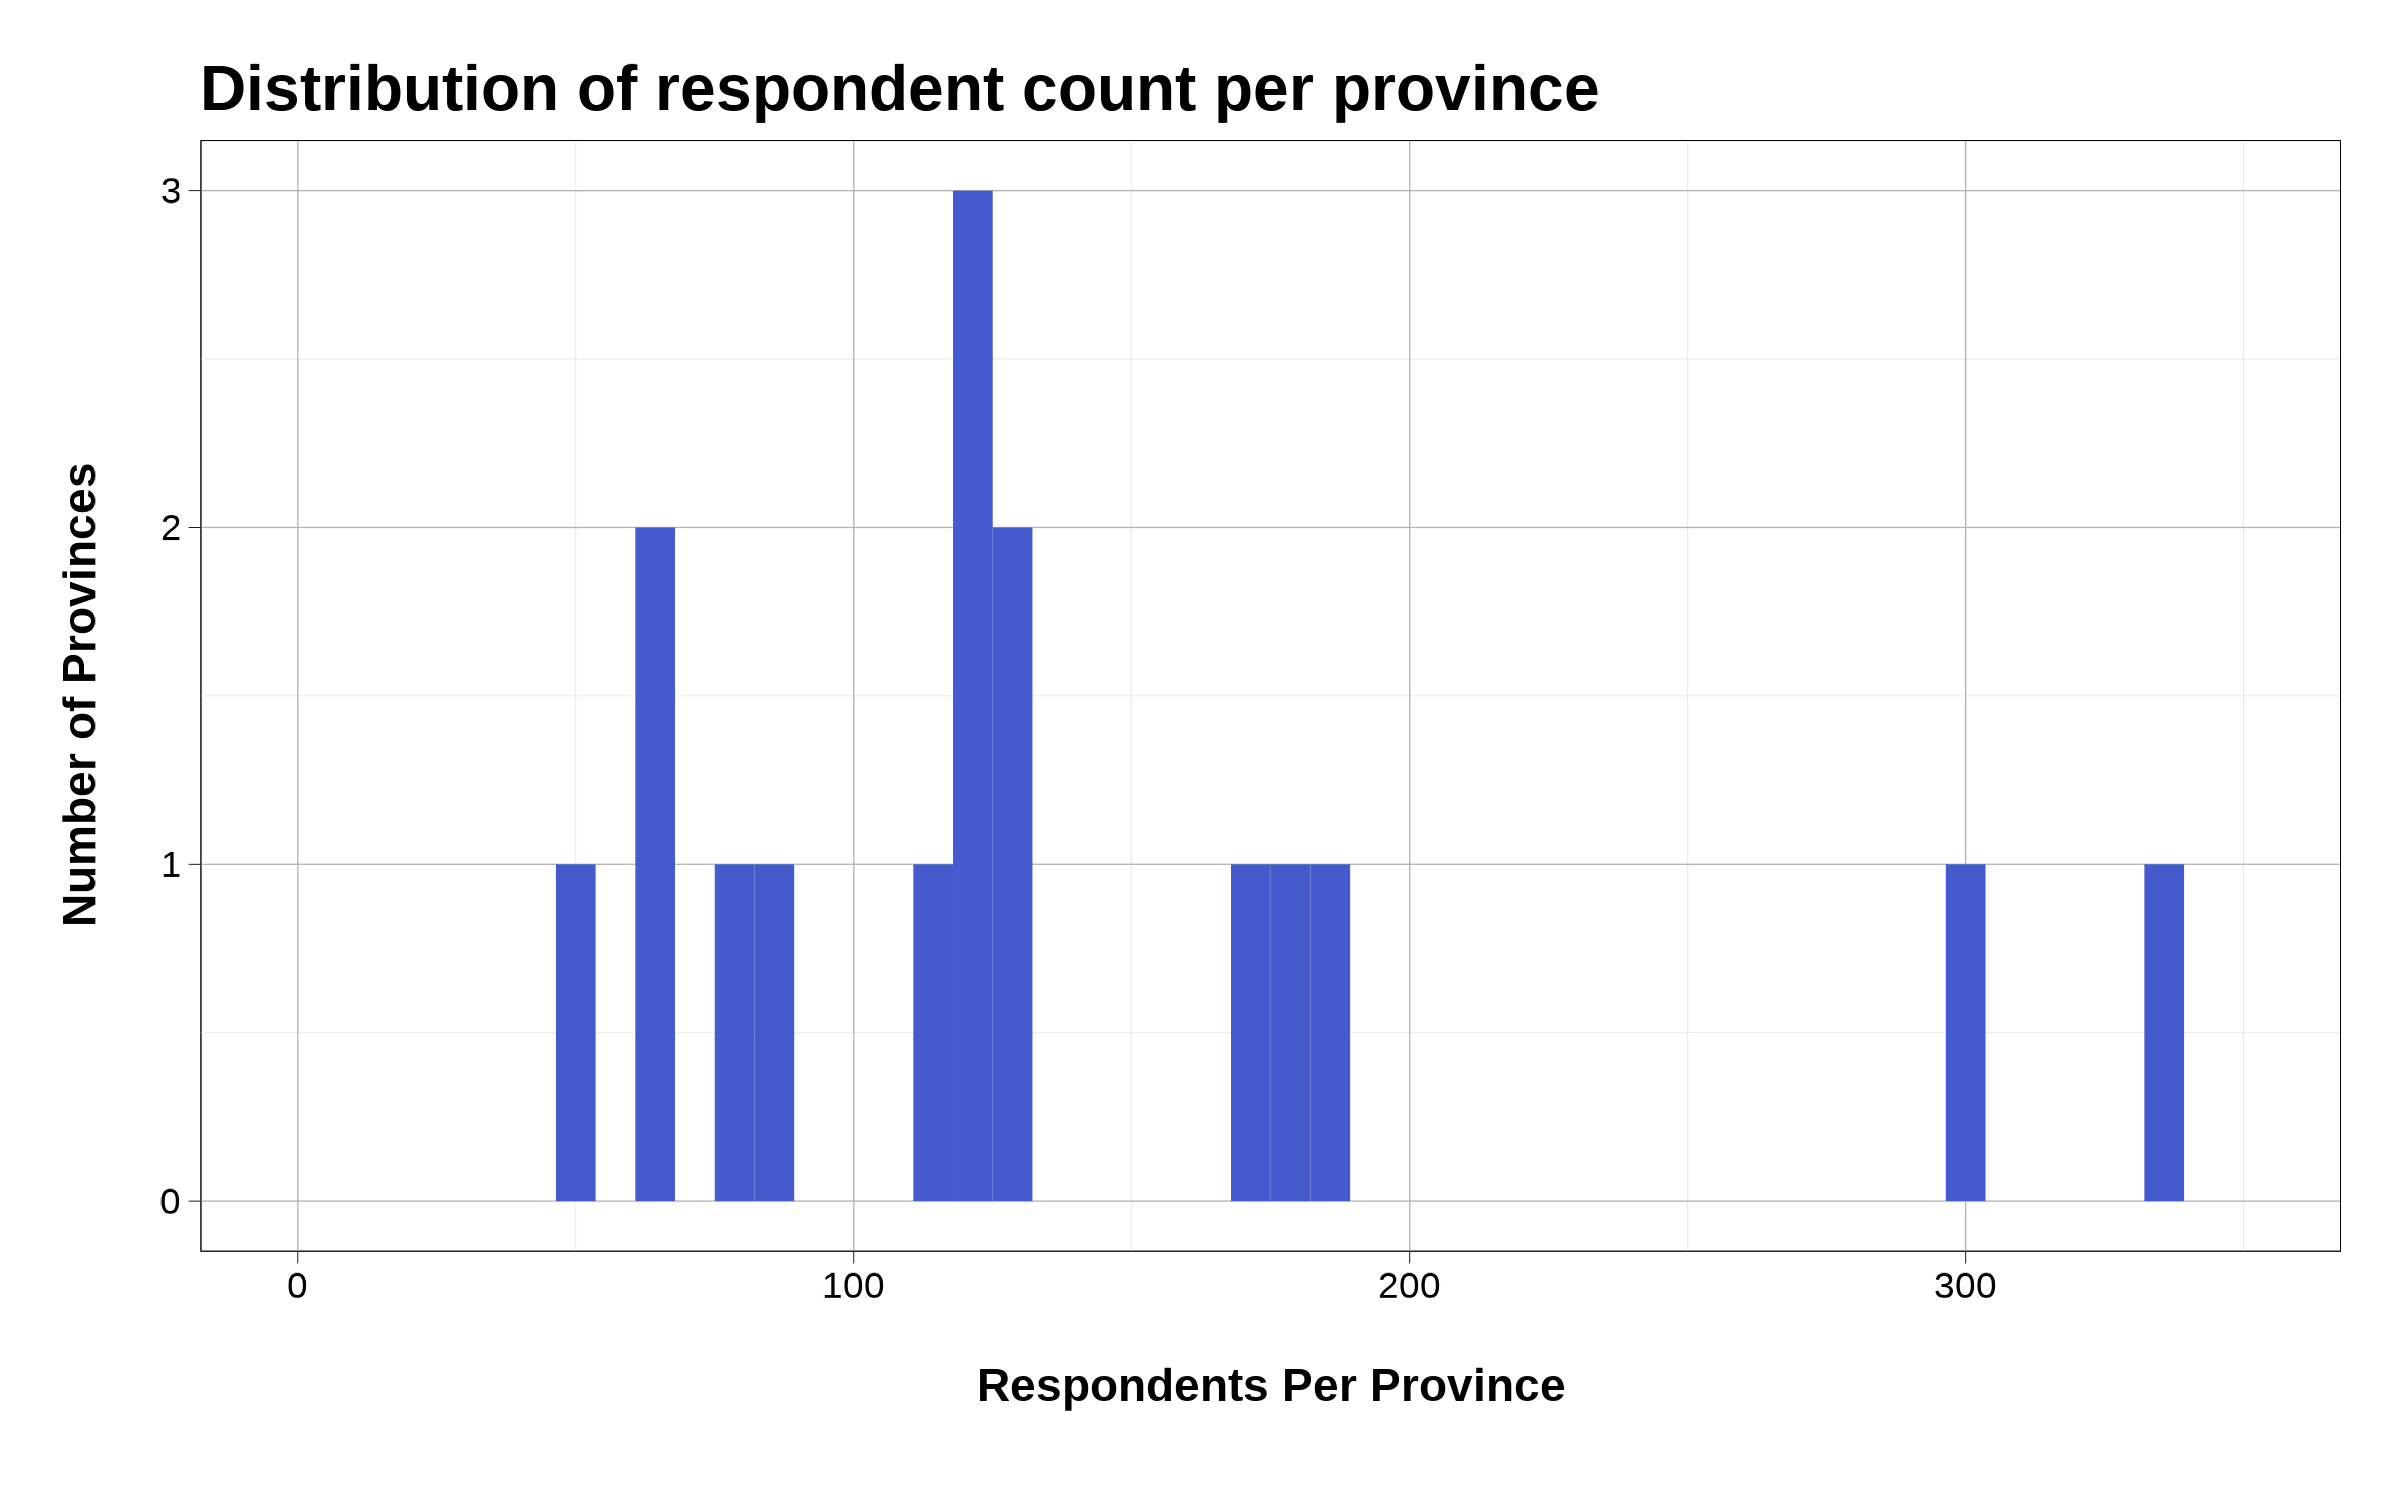
\includegraphics{../Figures/distribution-responses-province.png}

}

\caption{\label{fig-respondents-province}The number of survey
respondents per province.}

\end{figure}

Figure~\ref{fig-respondents-district} shows the number of respondents
per district---the lower level administrative unit below the province.
Here we can see substantial skew in the number of respondents per unit.
47 districts produce only one respondent. 64 districts only produce 2
respondents. At the other end of the distribution we have a few
districts that produce a vastly disproportionate share of our
respondents. 51 respondents come from Łódź, 54 from Poznań, and 150 come
from Warszawa. Though we run supplemental analyses using districts as a
grouping unit, we do not rely on these estimates to discuss variation in
attitudes as a function of geography.

\begin{figure}

{\centering 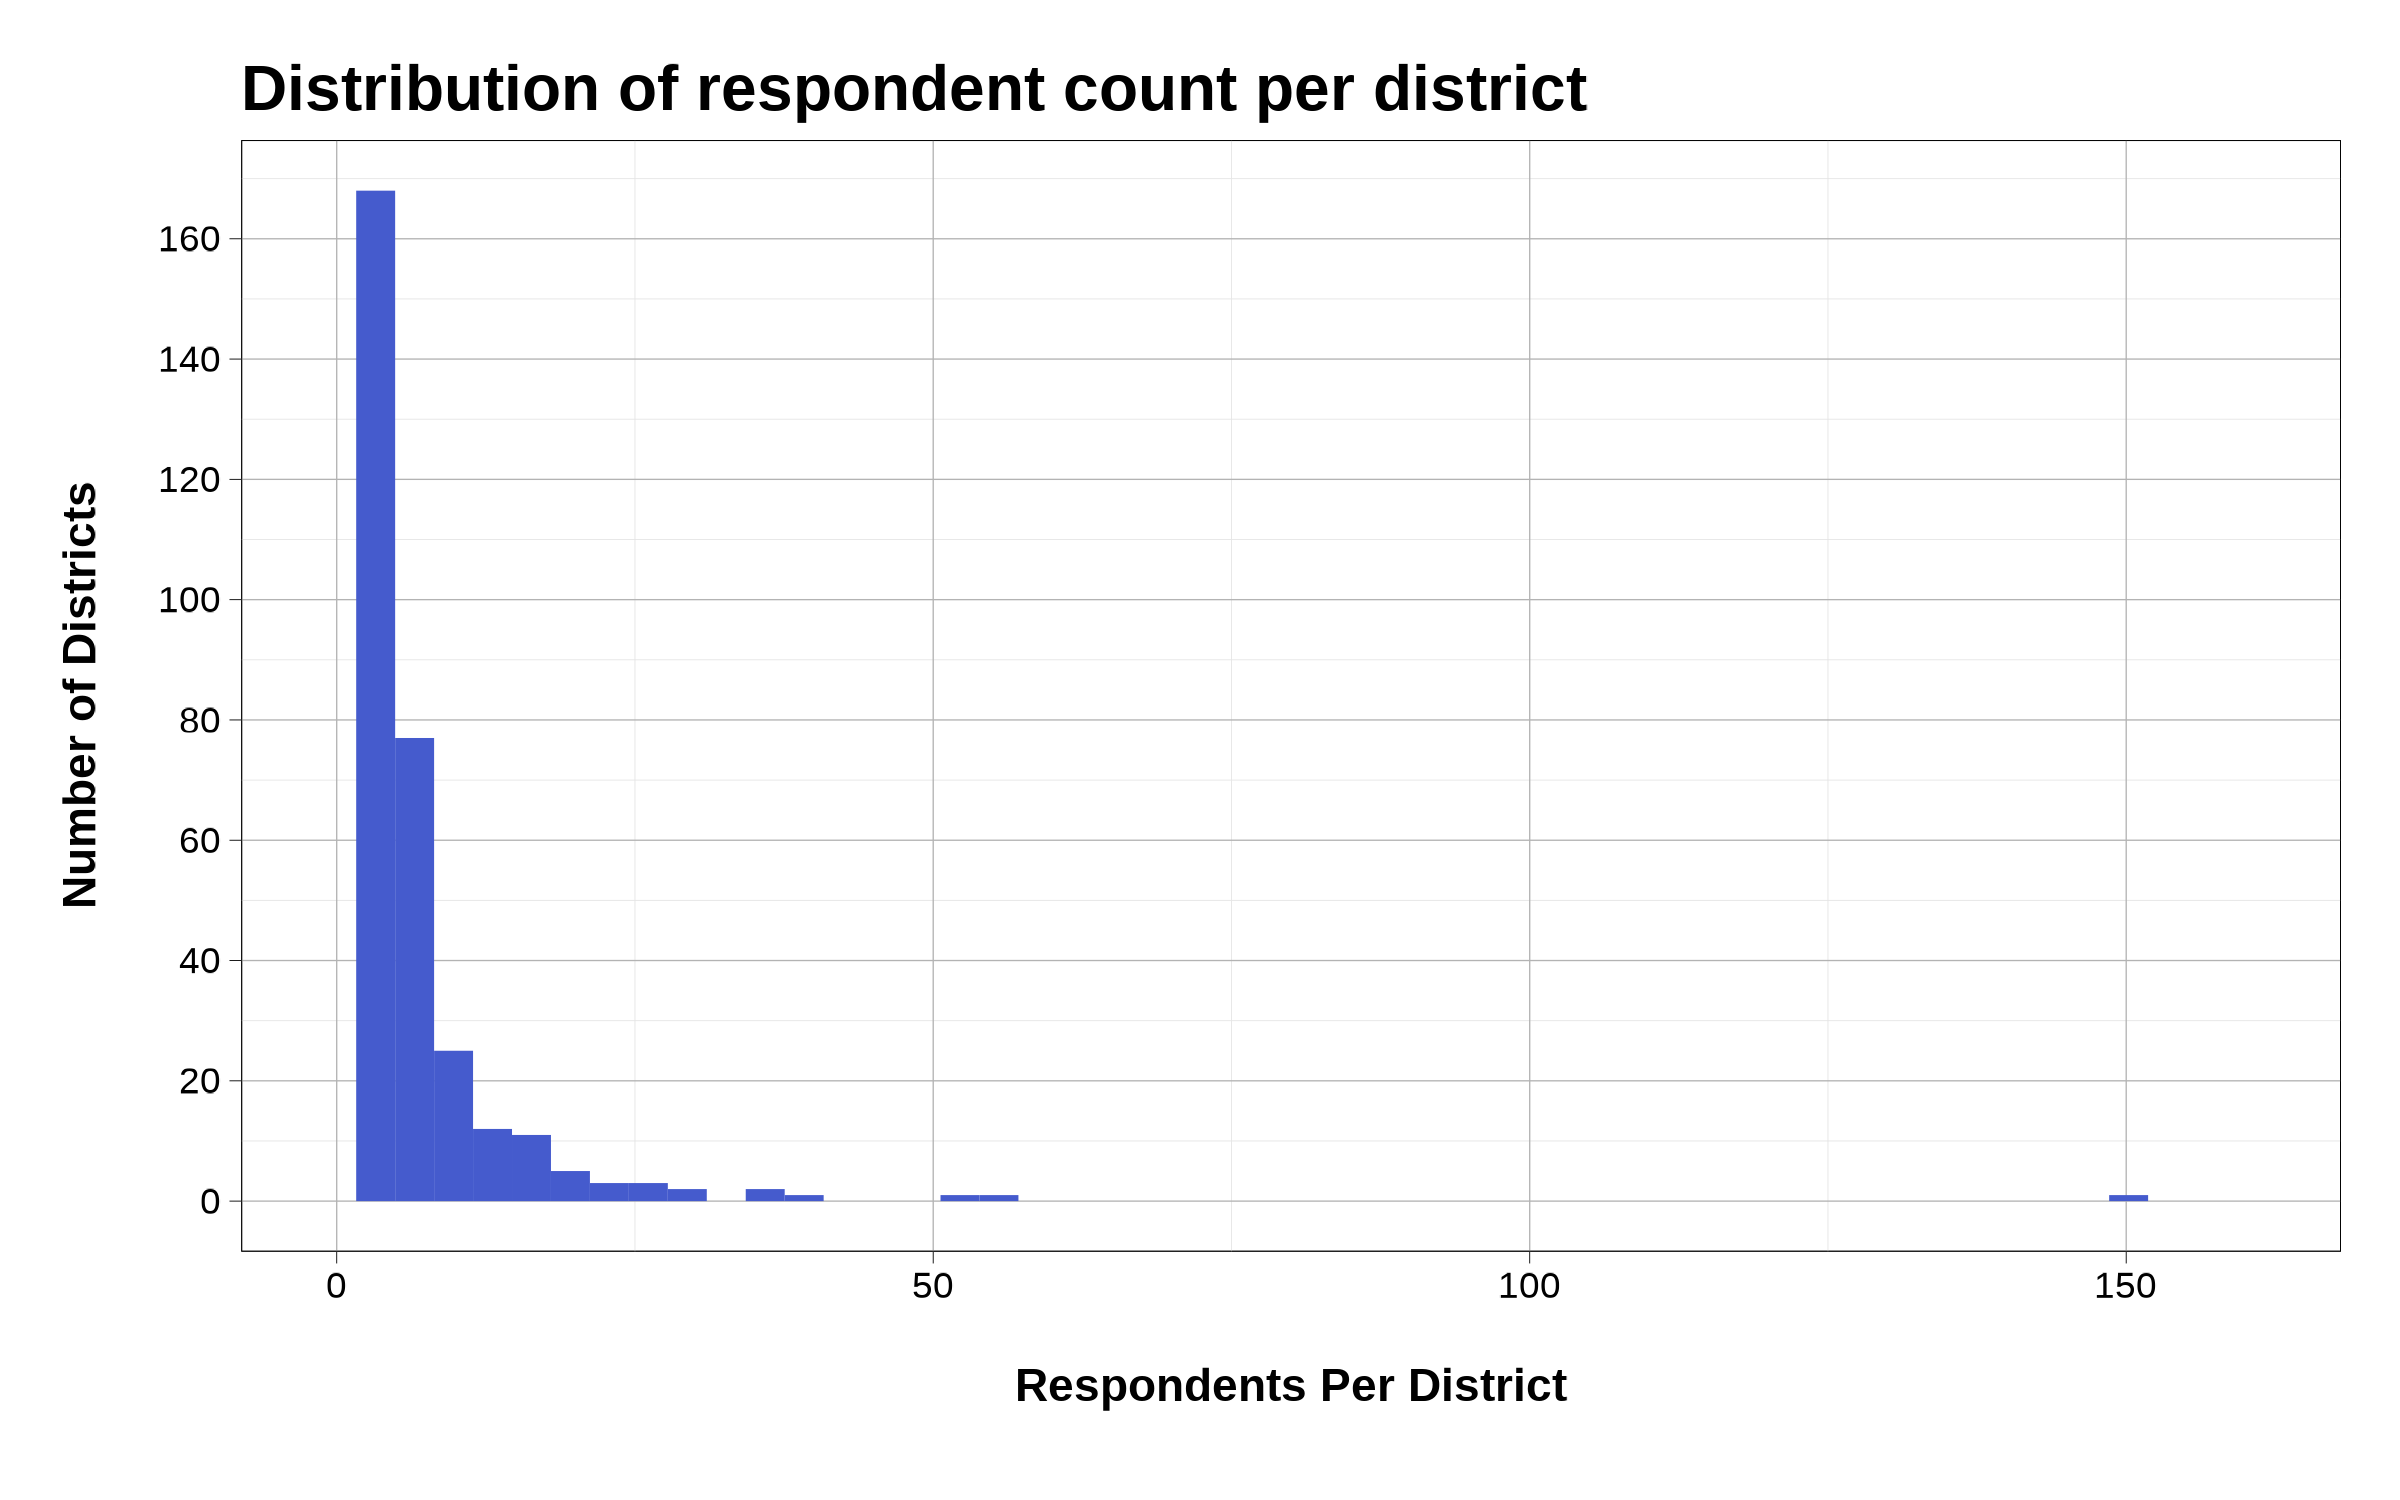
\includegraphics{../Figures/distribution-responses-district.png}

}

\caption{\label{fig-respondents-district}The number of survey
respondents per district.}

\end{figure}

\hypertarget{tables}{%
\section{Tables}\label{tables}}

This section contains a number of tables that provide descriptive
insights into the data, and information on the models we run for our
analysis.

\hypertarget{balance-tables}{%
\subsection{Balance Tables}\label{balance-tables}}

Table~\ref{tbl-balance-table} shows the balance of the predictor
variables across the four treatment groups in the experiment. Most of
the variables in our models are indicator variables, and so the numbers
shown in the columns correspond to the number of respondents who chose a
particular response for a particular question. For example, the number
of people who respond that they identify as either Male or Female.

The value in the parentheses indicates the percentage of responses that
fall into each of the four treatment categories. In general, we expect
this value to fall close to 25\% for each row.

Last, the final column shows the total number of responses for each
category/row.

We do not conduct a formal balance test, but this table helps us to
ensure that the randomization procedure worked as intended. In general,
we see most response-treatment groups falling at around the 25\% mark,
which is what we should expect if individuals were randomly assigned to
one of the four treatment categories. We see more substantial deviations
where the total number of observations for a given response is low. For
example, with only 40 total respondents indicating that their primary
income source was in the agricultural sector, small differences in the
number of people who fall into each treatment group have a larger effect
on the percentage value.

The final row shows the mean value and standard deviation (in
parentheses) for the ideology score, which is the only ordered integer
response variable we included in the survey. Since we mean-center this
measure, each category should have a mean of approximately 0 and a
standard deviation of 0.5.

\hypertarget{tbl-balance-table}{}
\begin{table}
\caption{\label{tbl-balance-table}Balance table for predictors used in primary models. }\tabularnewline

\centering\begingroup\fontsize{10}{12}\selectfont

\resizebox{\linewidth}{!}{
\begin{tabular}[t]{l|>{\raggedleft\arraybackslash}p{3.5cm}|>{\raggedleft\arraybackslash}p{3.5cm}|>{\raggedleft\arraybackslash}p{3.5cm}|>{\raggedleft\arraybackslash}p{3.5cm}|r}
\hline
\multicolumn{1}{l|}{ } & \multicolumn{4}{l|}{Treatment Group} & \multicolumn{1}{l}{ } \\
\cline{2-5}
Predictor Level & Control & Security & Economic & Security and Economic & All Groups\\
\hline
\multicolumn{6}{l}{\cellcolor[HTML]{3498DB}{\textcolor{white}{\textbf{Gender}}}}\\
\hline
\hspace{1em}\cellcolor{gray!6}{Male} & \cellcolor{gray!6}{273 (25.4\%)} & \cellcolor{gray!6}{270 (25.1\%)} & \cellcolor{gray!6}{267 (24.8\%)} & \cellcolor{gray!6}{265 (24.7\%)} & \cellcolor{gray!6}{1075}\\
\hline
\hspace{1em}Female & 284 (24.1\%) & 302 (25.7\%) & 288 (24.5\%) & 303 (25.7\%) & 1177\\
\hline
\hline
\hspace{1em}\cellcolor{gray!6}{None of the above} & \cellcolor{gray!6}{0 (0\%)} & \cellcolor{gray!6}{1 (50\%)} & \cellcolor{gray!6}{1 (50\%)} & \cellcolor{gray!6}{0 (0\%)} & \cellcolor{gray!6}{2}\\
\hline
\multicolumn{6}{l}{\cellcolor[HTML]{3498DB}{\textcolor{white}{\textbf{Minority}}}}\\
\hline
\hspace{1em}No & 456 (25.3\%) & 455 (25.2\%) & 449 (24.9\%) & 442 (24.5\%) & 1802\\
\hline
\hspace{1em}\cellcolor{gray!6}{Yes} & \cellcolor{gray!6}{84 (22.5\%)} & \cellcolor{gray!6}{94 (25.2\%)} & \cellcolor{gray!6}{92 (24.7\%)} & \cellcolor{gray!6}{103 (27.6\%)} & \cellcolor{gray!6}{373}\\
\hline
\hspace{1em}Decline to answer & 17 (21.5\%) & 24 (30.4\%) & 15 (19\%) & 23 (29.1\%) & 79\\
\hline
\multicolumn{6}{l}{\cellcolor[HTML]{3498DB}{\textcolor{white}{\textbf{Education}}}}\\
\hline
\hspace{1em}\cellcolor{gray!6}{Decline to answer} & \cellcolor{gray!6}{1 (20\%)} & \cellcolor{gray!6}{1 (20\%)} & \cellcolor{gray!6}{1 (20\%)} & \cellcolor{gray!6}{2 (40\%)} & \cellcolor{gray!6}{5}\\
\hline
\hspace{1em}Higher Education (Bachelor/Engineer) & 73 (23.2\%) & 74 (23.5\%) & 83 (26.3\%) & 85 (27\%) & 315\\
\hline
\hspace{1em}\cellcolor{gray!6}{Higher Education (Master’s degree or higher)} & \cellcolor{gray!6}{148 (24.7\%)} & \cellcolor{gray!6}{161 (26.9\%)} & \cellcolor{gray!6}{148 (24.7\%)} & \cellcolor{gray!6}{142 (23.7\%)} & \cellcolor{gray!6}{599}\\
\hline
\hspace{1em}Primary Education & 24 (34.8\%) & 19 (27.5\%) & 12 (17.4\%) & 14 (20.3\%) & 69\\
\hline
\hspace{1em}\cellcolor{gray!6}{Secondary Education} & \cellcolor{gray!6}{238 (25\%)} & \cellcolor{gray!6}{240 (25.2\%)} & \cellcolor{gray!6}{240 (25.2\%)} & \cellcolor{gray!6}{234 (24.6\%)} & \cellcolor{gray!6}{952}\\
\hline
\hspace{1em}Vocational School & 73 (23.2\%) & 78 (24.8\%) & 72 (22.9\%) & 91 (29\%) & 314\\
\hline
\multicolumn{6}{l}{\cellcolor[HTML]{3498DB}{\textcolor{white}{\textbf{Age}}}}\\
\hline
\hspace{1em}\cellcolor{gray!6}{18 to 24 years} & \cellcolor{gray!6}{58 (28.6\%)} & \cellcolor{gray!6}{50 (24.6\%)} & \cellcolor{gray!6}{41 (20.2\%)} & \cellcolor{gray!6}{54 (26.6\%)} & \cellcolor{gray!6}{203}\\
\hline
\hspace{1em}25 to 34 years & 114 (26.6\%) & 109 (25.5\%) & 108 (25.2\%) & 97 (22.7\%) & 428\\
\hline
\hspace{1em}\cellcolor{gray!6}{35 to 44 years} & \cellcolor{gray!6}{112 (23.7\%)} & \cellcolor{gray!6}{136 (28.8\%)} & \cellcolor{gray!6}{110 (23.3\%)} & \cellcolor{gray!6}{115 (24.3\%)} & \cellcolor{gray!6}{473}\\
\hline
\hspace{1em}45 to 54 years & 91 (23.6\%) & 85 (22.1\%) & 104 (27\%) & 105 (27.3\%) & 385\\
\hline
\hspace{1em}\cellcolor{gray!6}{55 to 64 years} & \cellcolor{gray!6}{115 (23.3\%)} & \cellcolor{gray!6}{133 (27\%)} & \cellcolor{gray!6}{120 (24.3\%)} & \cellcolor{gray!6}{125 (25.4\%)} & \cellcolor{gray!6}{493}\\
\hline
\hspace{1em}Age 65 or older & 67 (24.6\%) & 60 (22.1\%) & 73 (26.8\%) & 72 (26.5\%) & 272\\
\hline
\multicolumn{6}{l}{\cellcolor[HTML]{3498DB}{\textcolor{white}{\textbf{Income}}}}\\
\hline
\hspace{1em}\cellcolor{gray!6}{0 – 43 339} & \cellcolor{gray!6}{109 (25.6\%)} & \cellcolor{gray!6}{98 (23\%)} & \cellcolor{gray!6}{111 (26.1\%)} & \cellcolor{gray!6}{108 (25.4\%)} & \cellcolor{gray!6}{426}\\
\hline
\hspace{1em}43 340 – 57 187 & 85 (22.3\%) & 112 (29.4\%) & 82 (21.5\%) & 102 (26.8\%) & 381\\
\hline
\hspace{1em}\cellcolor{gray!6}{57 188 –  74 062} & \cellcolor{gray!6}{113 (25.1\%)} & \cellcolor{gray!6}{115 (25.6\%)} & \cellcolor{gray!6}{104 (23.1\%)} & \cellcolor{gray!6}{118 (26.2\%)} & \cellcolor{gray!6}{450}\\
\hline
\hspace{1em}74 063 – 93 937 & 105 (23.4\%) & 120 (26.7\%) & 118 (26.3\%) & 106 (23.6\%) & 449\\
\hline
\hspace{1em}\cellcolor{gray!6}{93 938 +} & \cellcolor{gray!6}{114 (25.3\%)} & \cellcolor{gray!6}{110 (24.4\%)} & \cellcolor{gray!6}{120 (26.7\%)} & \cellcolor{gray!6}{106 (23.6\%)} & \cellcolor{gray!6}{450}\\
\hline
\hspace{1em}Decline to answer & 31 (31.6\%) & 18 (18.4\%) & 21 (21.4\%) & 28 (28.6\%) & 98\\
\hline
\multicolumn{6}{l}{\cellcolor[HTML]{3498DB}{\textcolor{white}{\textbf{Income Source}}}}\\
\hline
\hspace{1em}\cellcolor{gray!6}{Agriculture} & \cellcolor{gray!6}{8 (20\%)} & \cellcolor{gray!6}{15 (37.5\%)} & \cellcolor{gray!6}{6 (15\%)} & \cellcolor{gray!6}{11 (27.5\%)} & \cellcolor{gray!6}{40}\\
\hline
\hspace{1em}Full-time or contract work in the government or public sector & 57 (28.9\%) & 49 (24.9\%) & 46 (23.4\%) & 45 (22.8\%) & 197\\
\hline
\hspace{1em}\cellcolor{gray!6}{Full-time or contract work in the private sector} & \cellcolor{gray!6}{304 (25.2\%)} & \cellcolor{gray!6}{300 (24.8\%)} & \cellcolor{gray!6}{301 (24.9\%)} & \cellcolor{gray!6}{303 (25.1\%)} & \cellcolor{gray!6}{1208}\\
\hline
\hspace{1em}Other sources & 56 (24.1\%) & 65 (28\%) & 54 (23.3\%) & 57 (24.6\%) & 232\\
\hline
\hspace{1em}\cellcolor{gray!6}{Pension or retirement} & \cellcolor{gray!6}{103 (22.5\%)} & \cellcolor{gray!6}{113 (24.7\%)} & \cellcolor{gray!6}{121 (26.5\%)} & \cellcolor{gray!6}{120 (26.3\%)} & \cellcolor{gray!6}{457}\\
\hline
\hspace{1em}Self-employed (non-agricultural) & 29 (24.2\%) & 31 (25.8\%) & 28 (23.3\%) & 32 (26.7\%) & 120\\
\hline
\multicolumn{6}{l}{\cellcolor[HTML]{3498DB}{\textcolor{white}{\textbf{Ideology}}}}\\
\hline
\hspace{1em}\cellcolor{gray!6}{Ideology} & \cellcolor{gray!6}{-0.024 (0.488)} & \cellcolor{gray!6}{0.02 (0.499)} & \cellcolor{gray!6}{0.006 (0.503)} & \cellcolor{gray!6}{-0.003 (0.51)} & \cellcolor{gray!6}{0 (0.5)}\\
\hline
\hline
\end{tabular}}
\endgroup{}
\end{table}

\hypertarget{model-tables}{%
\subsection{Model Tables}\label{model-tables}}

This section contains the tables for the models we run in our analysis.
All of the models were run using \texttt{brms} package version 2.19.0
{[}\citet{Burkner2017}; \citet{Burkner2018}; Stan2023{]}.

\begin{enumerate}
\def\labelenumi{\arabic{enumi}.}
\tightlist
\item
  Table~\ref{tbl-bivariate} shows the results of a multinomial logit
  model where we regress the outcome variable on the treatment group
  variable.
\item
  Table~\ref{tbl-base-model} shows the results of our primary
  multinomial multilevel logit model. This model regresses the outcome
  response onto the treatment variable and several other predictor
  variables. Varying intercepts by province.
\item
  Table~\ref{tbl-district-model} shows the results of our a multinomial
  multilevel logit model that regresses the outcome response onto the
  treatment variable and several other predictor variables. Varying
  intercepts by province and district.
\item
  Table~\ref{tbl-full-response} shows the results of a model where we
  use the full six category response variable rather than the four
  category response used in our primary models.
\item
  Table~\ref{tbl-varying} shows the results of a model that replicates
  our primary multilevel model, but allows the effects of the treatment
  variable to vary across province.
\item
  Table~\ref{tbl-treat-group} changes the basic model specification
  slightly and uses the treatment group as the grouping term for the
  varying intercepts. We also include a variable indicating whether the
  respondent reported having personal contact with a U.S. service
  member, and we allow this effect to vary across treatment groups.
\item
  Table~\ref{tbl-contact-int} builds upon our primary model in
  Table~\ref{tbl-base-model} by adding a variable indicating whether the
  respondent reported having personal contact with a U.S. service
  member, and an interaction term between the contact variable and the
  treatment. We also include varying intercepts on province.
\item
  Table~\ref{tbl-contact-int-district} replicates the models from
  Table~\ref{tbl-contact-int} but includes varying intercepts on both
  province and district.
\item
  Table~\ref{tbl-ordered} shows the results of a multilevel ordered
  logit model. Here we take the original six category response variable,
  drop the ``Don't know/Decline'' Responses, and treat the remaining
  responses as ordered from ``Strongly Oppose'' to ``Strongly Support''.
\end{enumerate}

\hypertarget{tbl-bivariate}{}
\begin{table}

\caption{\label{tbl-bivariate}Multinomial logistic regressions with treatment effects and outcome
response. Models only include the treatment received by the respondent
and their response. }Bivariate}
\centering
\fontsize{8}{10}\selectfont
\begin{tabular}[t]{lcccccc}
\toprule
\multicolumn{1}{c}{ } & \multicolumn{3}{c}{Distance: 100k} & \multicolumn{3}{c}{Distance: 5k} \\
\cmidrule(l{3pt}r{3pt}){2-4} \cmidrule(l{3pt}r{3pt}){5-7}
  & DKDA & Oppose & Support & DKDA & Oppose & Support\\
\midrule
\addlinespace[0.3em]
\multicolumn{7}{l}{\cellcolor[HTML]{3498DB}{\textbf{Treatment}}}\\
\hspace{1em}Economic & 5.851 & 0.202 & 0.243 & 0.467 & 0.004 & 0.063\\
\hspace{1em} & {}[2.680, 11.158] & {}[-0.301, 0.706] & {}[-0.091, 0.578] & {}[-0.186, 1.150] & {}[-0.373, 0.369] & {}[-0.250, 0.373]\\
\hspace{1em}Security & 5.300 & 0.486 & -0.035 & -0.053 & 0.356 & 0.017\\
\hspace{1em} & {}[2.102, 10.600] & {}[0.032, 0.951] & {}[-0.361, 0.284] & {}[-0.793, 0.676] & {}[-0.009, 0.713] & {}[-0.299, 0.328]\\
\hspace{1em}Security and Economic & 5.618 & 0.269 & 0.010 & -0.163 & 0.107 & 0.049\\
\hspace{1em} & {}[2.459, 10.901] & {}[-0.212, 0.758] & {}[-0.319, 0.339] & {}[-0.917, 0.576] & {}[-0.263, 0.475] & {}[-0.262, 0.360]\\
Intercept & -6.898 & -0.585 & 1.536 & -1.796 & 0.109 & 1.078\\
 & {}[-12.193, -3.786] & {}[-0.941, -0.240] & {}[1.313, 1.773] & {}[-2.328, -1.311] & {}[-0.146, 0.377] & {}[0.864, 1.298]\\
\midrule
N & 2239 &  &  & 2254 &  & \\
N.Groups & 0 &  &  & 0 &  & \\
\bottomrule
\end{tabular}
\end{table}

\hypertarget{tbl-base-model}{}
\begin{table}

\caption{\label{tbl-base-model}Multilevel multinomial logistic regressions with respondents grouped by
province. These model the response as a function of the treatment
variables and several predictor variables, with varying intercepts by
province. }Base Model}
\centering
\fontsize{8}{10}\selectfont
\begin{tabular}[t]{lcccccc}
\toprule
\multicolumn{1}{c}{ } & \multicolumn{3}{c}{Distance: 100k} & \multicolumn{3}{c}{Distance: 5k} \\
\cmidrule(l{3pt}r{3pt}){2-4} \cmidrule(l{3pt}r{3pt}){5-7}
  & DKDA & Oppose & Support & DKDA & Oppose & Support\\
\midrule
\addlinespace[0.3em]
\multicolumn{7}{l}{\cellcolor[HTML]{3498DB}{\textbf{Treatment}}}\\
\hspace{1em}Economic & 4.792 & 0.254 & 0.204 & 0.795 & 0.063 & 0.046\\
\hspace{1em} & {}[2.888, 7.351] & {}[-0.256, 0.760] & {}[-0.149, 0.558] & {}[0.088, 1.515] & {}[-0.320, 0.443] & {}[-0.280, 0.369]\\
\hspace{1em}Security & 3.948 & 0.584 & -0.062 & 0.140 & 0.433 & 0.019\\
\hspace{1em} & {}[2.017, 6.494] & {}[0.110, 1.053] & {}[-0.388, 0.277] & {}[-0.634, 0.915] & {}[0.070, 0.801] & {}[-0.304, 0.343]\\
\hspace{1em}Security and Economic & 4.359 & 0.325 & 0.002 & -0.080 & 0.170 & 0.085\\
\hspace{1em} & {}[2.457, 6.914] & {}[-0.162, 0.815] & {}[-0.337, 0.338] & {}[-0.894, 0.723] & {}[-0.207, 0.547] & {}[-0.240, 0.410]\\
\addlinespace[0.3em]
\multicolumn{7}{l}{\cellcolor[HTML]{3498DB}{\textbf{Age}}}\\
\hspace{1em}25-34 & -1.799 & -0.077 & -0.113 & -1.394 & -0.312 & -0.058\\
\hspace{1em} & {}[-2.346, -1.248] & {}[-0.404, 0.256] & {}[-0.375, 0.148] & {}[-1.928, -0.854] & {}[-0.605, -0.020] & {}[-0.315, 0.211]\\
\hspace{1em}35-44 & -1.988 & -0.310 & 0.039 & -1.496 & -0.617 & 0.045\\
\hspace{1em} & {}[-2.555, -1.435] & {}[-0.641, 0.019] & {}[-0.225, 0.304] & {}[-2.051, -0.949] & {}[-0.906, -0.330] & {}[-0.217, 0.310]\\
\hspace{1em}45-54 & -1.864 & -0.348 & 0.084 & -1.464 & -0.694 & 0.151\\
\hspace{1em} & {}[-2.473, -1.268] & {}[-0.699, 0.004] & {}[-0.198, 0.364] & {}[-2.047, -0.878] & {}[-1.006, -0.384] & {}[-0.127, 0.428]\\
\hspace{1em}55-64 & -1.785 & -0.441 & 0.462 & -1.549 & -0.925 & 0.413\\
\hspace{1em} & {}[-2.480, -1.096] & {}[-0.846, -0.040] & {}[0.150, 0.771] & {}[-2.205, -0.895] & {}[-1.266, -0.583] & {}[0.115, 0.716]\\
\hspace{1em}65+ & -2.525 & 0.194 & 0.655 & -2.230 & -0.496 & 0.564\\
\hspace{1em} & {}[-3.693, -1.367] & {}[-0.568, 0.943] & {}[0.135, 1.171] & {}[-3.291, -1.154] & {}[-1.093, 0.092] & {}[0.062, 1.070]\\
\addlinespace[0.3em]
\multicolumn{7}{l}{\cellcolor[HTML]{3498DB}{\textbf{Income}}}\\
\hspace{1em}Second Quantile & -0.905 & 0.022 & -0.103 & -0.914 & -0.038 & -0.106\\
\hspace{1em} & {}[-1.434, -0.374] & {}[-0.302, 0.342] & {}[-0.355, 0.146] & {}[-1.419, -0.410] & {}[-0.319, 0.244] & {}[-0.353, 0.143]\\
\hspace{1em}Third Quantile & -0.562 & 0.122 & -0.060 & -0.709 & 0.076 & -0.030\\
\hspace{1em} & {}[-1.074, -0.047] & {}[-0.195, 0.440] & {}[-0.309, 0.194] & {}[-1.206, -0.210] & {}[-0.200, 0.353] & {}[-0.271, 0.212]\\
\hspace{1em}Fourth Quantile & -0.910 & 0.012 & 0.050 & -0.949 & -0.024 & -0.041\\
\hspace{1em} & {}[-1.494, -0.328] & {}[-0.334, 0.354] & {}[-0.211, 0.312] & {}[-1.505, -0.402] & {}[-0.317, 0.274] & {}[-0.299, 0.218]\\
\hspace{1em}Fifth Quantile & -0.757 & 0.111 & 0.178 & -0.778 & 0.035 & 0.137\\
\hspace{1em} & {}[-1.434, -0.084] & {}[-0.276, 0.506] & {}[-0.116, 0.475] & {}[-1.429, -0.133] & {}[-0.294, 0.358] & {}[-0.148, 0.422]\\
\hspace{1em}Income Decline & -0.317 & 0.636 & -0.124 & 0.302 & 0.238 & -0.318\\
\hspace{1em} & {}[-1.583, 0.892] & {}[-0.189, 1.455] & {}[-0.755, 0.539] & {}[-0.660, 1.245] & {}[-0.410, 0.893] & {}[-0.934, 0.303]\\
\addlinespace[0.3em]
\multicolumn{7}{l}{\cellcolor[HTML]{3498DB}{\textbf{Income Source}}}\\
\hspace{1em}Public sector contract work & 1.335 & 0.137 & 0.643 & -0.237 & 0.094 & 0.870\\
\hspace{1em} & {}[-1.122, 4.249] & {}[-1.099, 1.422] & {}[-0.311, 1.546] & {}[-1.944, 1.612] & {}[-0.885, 1.074] & {}[-0.057, 1.780]\\
\hspace{1em}Private sector contract work & 1.406 & 0.105 & 0.629 & -0.214 & 0.261 & 1.020\\
\hspace{1em} & {}[-0.822, 4.256] & {}[-1.005, 1.258] & {}[-0.234, 1.434] & {}[-1.693, 1.468] & {}[-0.631, 1.146] & {}[0.154, 1.864]\\
\hspace{1em}Pension or Retirement & 2.590 & -0.179 & 0.573 & 1.198 & 0.209 & 1.134\\
\hspace{1em} & {}[0.178, 5.569] & {}[-1.449, 1.148] & {}[-0.377, 1.470] & {}[-0.425, 2.980] & {}[-0.805, 1.228] & {}[0.196, 2.064]\\
\hspace{1em}Self-employed (non-agricultural) & -0.049 & -0.320 & 0.390 & -1.259 & 0.213 & 1.104\\
\hspace{1em} & {}[-3.478, 3.383] & {}[-1.648, 1.035] & {}[-0.583, 1.332] & {}[-4.175, 1.228] & {}[-0.832, 1.274] & {}[0.121, 2.074]\\
\hspace{1em}Other sources & 1.887 & 0.090 & 0.574 & -0.151 & -0.153 & 0.429\\
\hspace{1em} & {}[-0.377, 4.761] & {}[-1.083, 1.308] & {}[-0.337, 1.441] & {}[-1.678, 1.553] & {}[-1.092, 0.774] & {}[-0.494, 1.324]\\
\addlinespace[0.3em]
\multicolumn{7}{l}{\cellcolor[HTML]{3498DB}{\textbf{Education}}}\\
\hspace{1em}Bachelor's degree or Engineer & 0.767 & 0.474 & 1.933 & 3.473 & 0.157 & 5.177\\
\hspace{1em} & {}[-2.595, 4.253] & {}[-2.510, 3.915] & {}[-0.983, 5.347] & {}[-1.098, 11.490] & {}[-2.067, 2.515] & {}[-0.157, 15.042]\\
\hspace{1em}Master's degree or higher & 0.833 & 0.253 & 1.647 & 3.001 & 0.371 & 5.408\\
\hspace{1em} & {}[-2.492, 4.354] & {}[-2.715, 3.672] & {}[-1.290, 5.022] & {}[-1.593, 11.073] & {}[-1.839, 2.710] & {}[0.068, 15.253]\\
\hspace{1em}Primary Education & 1.975 & 0.078 & 2.134 & 5.457 & 1.176 & 6.356\\
\hspace{1em} & {}[-1.477, 5.517] & {}[-3.134, 3.639] & {}[-0.888, 5.591] & {}[0.876, 13.530] & {}[-1.198, 3.678] & {}[0.920, 16.198]\\
\hspace{1em}Secondary Education & 0.345 & 0.305 & 1.588 & 3.281 & 0.458 & 5.311\\
\hspace{1em} & {}[-2.926, 3.776] & {}[-2.650, 3.697] & {}[-1.339, 4.941] & {}[-1.201, 11.283] & {}[-1.737, 2.782] & {}[-0.015, 15.176]\\
\hspace{1em}Vocational School & 0.921 & 0.284 & 1.335 & 3.684 & 0.365 & 5.071\\
\hspace{1em} & {}[-2.358, 4.357] & {}[-2.686, 3.706] & {}[-1.601, 4.710] & {}[-0.791, 11.703] & {}[-1.837, 2.701] & {}[-0.233, 14.901]\\
\addlinespace[0.3em]
\multicolumn{7}{l}{\cellcolor[HTML]{3498DB}{\textbf{Ideology}}}\\
\hspace{1em}Ideology & -0.298 & -0.372 & 0.597 & -0.320 & -0.302 & 0.567\\
\hspace{1em} & {}[-0.541, -0.057] & {}[-0.498, -0.246] & {}[0.491, 0.703] & {}[-0.566, -0.074] & {}[-0.421, -0.184] & {}[0.460, 0.674]\\
\addlinespace[0.3em]
\multicolumn{7}{l}{\cellcolor[HTML]{3498DB}{\textbf{Minority}}}\\
\hspace{1em}Minority: Yes & 0.188 & 0.058 & -0.213 & -0.039 & -0.070 & -0.214\\
\hspace{1em} & {}[-0.214, 0.595] & {}[-0.157, 0.273] & {}[-0.380, -0.043] & {}[-0.436, 0.351] & {}[-0.262, 0.123] & {}[-0.381, -0.045]\\
\hspace{1em}Minority: Decline & 2.044 & -0.221 & -0.450 & 1.106 & -0.583 & -0.594\\
\hspace{1em} & {}[1.311, 2.765] & {}[-0.877, 0.424] & {}[-0.947, 0.052] & {}[0.396, 1.794] & {}[-1.150, -0.024] & {}[-1.095, -0.093]\\
\addlinespace[0.3em]
\multicolumn{7}{l}{\cellcolor[HTML]{3498DB}{\textbf{Gender}}}\\
\hspace{1em}Female & 0.605 & -0.111 & -0.402 & 0.660 & 0.013 & -0.394\\
\hspace{1em} & {}[0.361, 0.849] & {}[-0.243, 0.021] & {}[-0.506, -0.298] & {}[0.423, 0.897] & {}[-0.105, 0.131] & {}[-0.496, -0.294]\\
\hspace{1em}None of the Above & -12.237 & -0.774 & -23.846 & -12.495 & -0.590 & -23.047\\
\hspace{1em} & {}[-37.690, 1.661] & {}[-4.638, 3.041] & {}[-48.109, -3.720] & {}[-37.985, 1.731] & {}[-4.563, 3.202] & {}[-47.732, -2.780]\\
\addlinespace[0.3em]
\multicolumn{7}{l}{\cellcolor[HTML]{3498DB}{\textbf{Intercept}}}\\
\hspace{1em}Intercept & -6.835 & -0.850 & -0.530 & -4.417 & -0.009 & -5.081\\
\hspace{1em} & {}[-11.745, -2.335] & {}[-4.447, 2.349] & {}[-3.986, 2.540] & {}[-12.570, 0.413] & {}[-2.508, 2.368] & {}[-14.905, 0.304]\\
\midrule
N & 2239 &  &  & 2254 &  & \\
N.Groups & 16 &  &  & 16 &  & \\
Groups & province &  &  & province &  & \\
\bottomrule
\end{tabular}
\end{table}

\hypertarget{tbl-district-model}{}
\begin{table}

\caption{\label{tbl-district-model}Multilevel multinomial logistic regressions with respondents grouped by
province and district. These model the response as a function of the
treatment variables and several predictor variables, with varying
intercepts by province and by district. }District Model}
\centering
\fontsize{8}{10}\selectfont
\begin{tabular}[t]{lcccccc}
\toprule
\multicolumn{1}{c}{ } & \multicolumn{3}{c}{Distance: 100k} & \multicolumn{3}{c}{Distance: 5k} \\
\cmidrule(l{3pt}r{3pt}){2-4} \cmidrule(l{3pt}r{3pt}){5-7}
  & DKDA & Oppose & Support & DKDA & Oppose & Support\\
\midrule
\addlinespace[0.3em]
\multicolumn{7}{l}{\cellcolor[HTML]{3498DB}{\textbf{Treatment}}}\\
\hspace{1em}Economic & 5.037 & 0.255 & 0.212 & 0.905 & 0.047 & 0.038\\
\hspace{1em} & {}[3.065, 7.616] & {}[-0.268, 0.774] & {}[-0.144, 0.565] & {}[0.152, 1.681] & {}[-0.336, 0.430] & {}[-0.287, 0.369]\\
\hspace{1em}Security & 4.039 & 0.587 & -0.065 & 0.153 & 0.429 & 0.012\\
\hspace{1em} & {}[2.081, 6.574] & {}[0.100, 1.063] & {}[-0.405, 0.277] & {}[-0.660, 0.965] & {}[0.060, 0.802] & {}[-0.313, 0.337]\\
\hspace{1em}Security and Economic & 4.569 & 0.332 & 0.006 & -0.023 & 0.186 & 0.092\\
\hspace{1em} & {}[2.630, 7.109] & {}[-0.159, 0.831] & {}[-0.338, 0.346] & {}[-0.846, 0.804] & {}[-0.190, 0.565] & {}[-0.230, 0.421]\\
\addlinespace[0.3em]
\multicolumn{7}{l}{\cellcolor[HTML]{3498DB}{\textbf{Age}}}\\
\hspace{1em}25-34 & -1.931 & -0.066 & -0.104 & -1.497 & -0.298 & -0.053\\
\hspace{1em} & {}[-2.518, -1.351] & {}[-0.391, 0.258] & {}[-0.367, 0.159] & {}[-2.058, -0.935] & {}[-0.599, 0.002] & {}[-0.320, 0.213]\\
\hspace{1em}35-44 & -2.134 & -0.299 & 0.048 & -1.625 & -0.602 & 0.053\\
\hspace{1em} & {}[-2.730, -1.540] & {}[-0.624, 0.033] & {}[-0.217, 0.312] & {}[-2.201, -1.055] & {}[-0.901, -0.311] & {}[-0.215, 0.319]\\
\hspace{1em}45-54 & -2.003 & -0.340 & 0.096 & -1.573 & -0.683 & 0.158\\
\hspace{1em} & {}[-2.644, -1.379] & {}[-0.690, 0.008] & {}[-0.186, 0.376] & {}[-2.187, -0.970] & {}[-0.999, -0.369] & {}[-0.123, 0.441]\\
\hspace{1em}55-64 & -1.948 & -0.426 & 0.472 & -1.675 & -0.909 & 0.420\\
\hspace{1em} & {}[-2.692, -1.220] & {}[-0.824, -0.016] & {}[0.166, 0.785] & {}[-2.368, -0.989] & {}[-1.257, -0.560] & {}[0.116, 0.726]\\
\hspace{1em}65+ & -2.744 & 0.217 & 0.668 & -2.361 & -0.481 & 0.571\\
\hspace{1em} & {}[-3.979, -1.498] & {}[-0.540, 0.977] & {}[0.137, 1.194] & {}[-3.493, -1.240] & {}[-1.087, 0.128] & {}[0.062, 1.074]\\
\addlinespace[0.3em]
\multicolumn{7}{l}{\cellcolor[HTML]{3498DB}{\textbf{Income}}}\\
\hspace{1em}Second Quantile & -0.877 & 0.021 & -0.096 & -0.928 & -0.028 & -0.101\\
\hspace{1em} & {}[-1.412, -0.330] & {}[-0.307, 0.352] & {}[-0.346, 0.156] & {}[-1.445, -0.408] & {}[-0.308, 0.255] & {}[-0.351, 0.149]\\
\hspace{1em}Third Quantile & -0.530 & 0.121 & -0.057 & -0.712 & 0.087 & -0.024\\
\hspace{1em} & {}[-1.065, 0.000] & {}[-0.194, 0.444] & {}[-0.307, 0.192] & {}[-1.216, -0.210] & {}[-0.193, 0.366] & {}[-0.267, 0.219]\\
\hspace{1em}Fourth Quantile & -0.848 & 0.008 & 0.057 & -0.927 & -0.017 & -0.034\\
\hspace{1em} & {}[-1.436, -0.256] & {}[-0.340, 0.360] & {}[-0.211, 0.327] & {}[-1.503, -0.357] & {}[-0.313, 0.280] & {}[-0.294, 0.224]\\
\hspace{1em}Fifth Quantile & -0.688 & 0.109 & 0.186 & -0.753 & 0.036 & 0.142\\
\hspace{1em} & {}[-1.381, 0.004] & {}[-0.279, 0.499] & {}[-0.110, 0.480] & {}[-1.419, -0.072] & {}[-0.288, 0.361] & {}[-0.144, 0.426]\\
\hspace{1em}Income Decline & -0.134 & 0.647 & -0.107 & 0.391 & 0.260 & -0.307\\
\hspace{1em} & {}[-1.456, 1.150] & {}[-0.183, 1.491] & {}[-0.748, 0.569] & {}[-0.629, 1.387] & {}[-0.405, 0.928] & {}[-0.925, 0.326]\\
\addlinespace[0.3em]
\multicolumn{7}{l}{\cellcolor[HTML]{3498DB}{\textbf{Income Source}}}\\
\hspace{1em}Public sector contract work & 1.285 & 0.127 & 0.645 & -0.395 & 0.105 & 0.855\\
\hspace{1em} & {}[-1.308, 4.365] & {}[-1.118, 1.427] & {}[-0.308, 1.562] & {}[-2.208, 1.562] & {}[-0.915, 1.114] & {}[-0.079, 1.776]\\
\hspace{1em}Private sector contract work & 1.205 & 0.101 & 0.633 & -0.451 & 0.272 & 1.005\\
\hspace{1em} & {}[-1.199, 4.170] & {}[-1.011, 1.271] & {}[-0.249, 1.446] & {}[-2.034, 1.330] & {}[-0.657, 1.186] & {}[0.136, 1.867]\\
\hspace{1em}Pension or Retirement & 2.484 & -0.200 & 0.578 & 1.014 & 0.214 & 1.125\\
\hspace{1em} & {}[-0.065, 5.559] & {}[-1.499, 1.126] & {}[-0.389, 1.507] & {}[-0.702, 2.902] & {}[-0.830, 1.243] & {}[0.196, 2.068]\\
\hspace{1em}Self-employed (non-agricultural) & -0.359 & -0.350 & 0.376 & -1.442 & 0.239 & 1.099\\
\hspace{1em} & {}[-3.890, 3.151] & {}[-1.665, 1.004] & {}[-0.614, 1.326] & {}[-4.449, 1.091] & {}[-0.856, 1.322] & {}[0.103, 2.100]\\
\hspace{1em}Other sources & 1.715 & 0.082 & 0.580 & -0.349 & -0.138 & 0.424\\
\hspace{1em} & {}[-0.712, 4.694] & {}[-1.105, 1.305] & {}[-0.358, 1.461] & {}[-1.953, 1.459] & {}[-1.123, 0.841] & {}[-0.493, 1.334]\\
\addlinespace[0.3em]
\multicolumn{7}{l}{\cellcolor[HTML]{3498DB}{\textbf{Education}}}\\
\hspace{1em}Bachelor's degree or Engineer & 0.571 & 0.485 & 1.928 & 3.797 & 0.063 & 5.016\\
\hspace{1em} & {}[-3.097, 4.342] & {}[-2.531, 3.976] & {}[-0.951, 5.229] & {}[-1.151, 12.212] & {}[-2.202, 2.424] & {}[-0.182, 14.701]\\
\hspace{1em}Master's degree or higher & 0.551 & 0.261 & 1.630 & 3.286 & 0.282 & 5.247\\
\hspace{1em} & {}[-3.126, 4.323] & {}[-2.726, 3.758] & {}[-1.226, 4.864] & {}[-1.688, 11.707] & {}[-1.969, 2.642] & {}[0.047, 14.902]\\
\hspace{1em}Primary Education & 2.030 & 0.064 & 2.154 & 5.849 & 1.099 & 6.217\\
\hspace{1em} & {}[-1.758, 5.939] & {}[-3.137, 3.734] & {}[-0.764, 5.517] & {}[0.828, 14.299] & {}[-1.309, 3.622] & {}[0.895, 15.911]\\
\hspace{1em}Secondary Education & 0.039 & 0.311 & 1.577 & 3.541 & 0.366 & 5.153\\
\hspace{1em} & {}[-3.546, 3.762] & {}[-2.671, 3.793] & {}[-1.284, 4.826] & {}[-1.400, 11.966] & {}[-1.862, 2.719] & {}[-0.019, 14.791]\\
\hspace{1em}Vocational School & 0.744 & 0.293 & 1.336 & 4.052 & 0.252 & 4.908\\
\hspace{1em} & {}[-2.836, 4.423] & {}[-2.708, 3.747] & {}[-1.538, 4.618] & {}[-0.831, 12.499] & {}[-2.001, 2.615] & {}[-0.298, 14.578]\\
\addlinespace[0.3em]
\multicolumn{7}{l}{\cellcolor[HTML]{3498DB}{\textbf{Ideology}}}\\
\hspace{1em}Ideology & -0.314 & -0.373 & 0.600 & -0.328 & -0.303 & 0.570\\
\hspace{1em} & {}[-0.565, -0.063] & {}[-0.499, -0.249] & {}[0.495, 0.706] & {}[-0.572, -0.084] & {}[-0.419, -0.185] & {}[0.466, 0.674]\\
\addlinespace[0.3em]
\multicolumn{7}{l}{\cellcolor[HTML]{3498DB}{\textbf{Minority}}}\\
\hspace{1em}Minority: Yes & 0.188 & 0.059 & -0.214 & -0.037 & -0.068 & -0.215\\
\hspace{1em} & {}[-0.220, 0.595] & {}[-0.157, 0.272] & {}[-0.384, -0.044] & {}[-0.439, 0.359] & {}[-0.264, 0.127] & {}[-0.382, -0.048]\\
\hspace{1em}Minority: Decline & 2.292 & -0.234 & -0.479 & 1.306 & -0.618 & -0.610\\
\hspace{1em} & {}[1.499, 3.103] & {}[-0.909, 0.414] & {}[-0.980, 0.030] & {}[0.538, 2.066] & {}[-1.190, -0.052] & {}[-1.110, -0.109]\\
\addlinespace[0.3em]
\multicolumn{7}{l}{\cellcolor[HTML]{3498DB}{\textbf{Gender}}}\\
\hspace{1em}Female & 0.597 & -0.110 & -0.400 & 0.666 & 0.011 & -0.394\\
\hspace{1em} & {}[0.348, 0.842] & {}[-0.244, 0.022] & {}[-0.504, -0.295] & {}[0.429, 0.905] & {}[-0.107, 0.128] & {}[-0.495, -0.294]\\
\hspace{1em}None of the Above & -12.133 & -0.821 & -23.909 & -12.448 & -0.534 & -22.982\\
\hspace{1em} & {}[-38.650, 2.220] & {}[-4.802, 3.075] & {}[-48.643, -3.721] & {}[-38.251, 1.763] & {}[-4.339, 3.167] & {}[-48.142, -2.411]\\
\addlinespace[0.3em]
\multicolumn{7}{l}{\cellcolor[HTML]{3498DB}{\textbf{Intercept}}}\\
\hspace{1em}Intercept & -7.043 & -0.895 & -0.532 & -4.863 & 0.026 & -4.910\\
\hspace{1em} & {}[-12.244, -2.297] & {}[-4.560, 2.318] & {}[-3.871, 2.418] & {}[-13.382, 0.380] & {}[-2.504, 2.432] & {}[-14.558, 0.375]\\
\midrule
N & 2239 &  &  & 2254 &  & \\
N.Groups & 16 &  &  & 16 &  & \\
Groups & province, province:district &  &  & province, province:district &  & \\
\bottomrule
\end{tabular}
\end{table}

\hypertarget{tbl-full-response}{}
\begin{table}

\caption{\label{tbl-full-response}Multilevel multinomial logistic regressions with respondents grouped by
province. These model the response as a function of the treatment
variables and several predictor variables, with varying intercepts by
province. Here we use the original six response categories rather than
the four aggregated categories from the main model. }Full Response Variable}
\centering
\fontsize{8}{10}\selectfont
\begin{tabular}[t]{lcccccccccc}
\toprule
\multicolumn{1}{c}{ } & \multicolumn{5}{c}{Distance: 100k} & \multicolumn{5}{c}{Distance: 5k} \\
\cmidrule(l{3pt}r{3pt}){2-6} \cmidrule(l{3pt}r{3pt}){7-11}
  & Stronglysupport & Somewhatsupport & Somewhatoppose & Stronglyoppose & DKDA & Stronglysupport & Somewhatsupport & Somewhatoppose & Stronglyoppose & DKDA\\
\midrule
\addlinespace[0.3em]
\multicolumn{11}{l}{\cellcolor[HTML]{3498DB}{\textbf{Treatment}}}\\
\hspace{1em}Economic & 0.162 & 0.239 & -0.013 & 0.439 & 5.533 & -0.004 & 0.049 & 0.115 & -0.078 & 0.561\\
\hspace{1em} & {}[-0.228, 0.552] & {}[-0.139, 0.620] & {}[-0.668, 0.637] & {}[-0.240, 1.118] & {}[2.733, 9.945] & {}[-0.385, 0.372] & {}[-0.308, 0.405] & {}[-0.340, 0.568] & {}[-0.558, 0.393] & {}[-0.131, 1.266]\\
\hspace{1em}Security & 0.094 & -0.186 & 0.369 & 0.753 & 4.796 & 0.138 & -0.073 & 0.426 & 0.406 & -0.064\\
\hspace{1em} & {}[-0.284, 0.472] & {}[-0.560, 0.193] & {}[-0.216, 0.963] & {}[0.123, 1.395] & {}[1.971, 9.200] & {}[-0.233, 0.509] & {}[-0.443, 0.298] & {}[-0.012, 0.870] & {}[-0.039, 0.860] & {}[-0.833, 0.707]\\
\hspace{1em}Security and Economic & 0.113 & -0.075 & 0.047 & 0.560 & 5.253 & 0.225 & -0.047 & 0.192 & 0.095 & -0.172\\
\hspace{1em} & {}[-0.257, 0.481] & {}[-0.441, 0.294] & {}[-0.567, 0.653] & {}[-0.078, 1.228] & {}[2.454, 9.665] & {}[-0.141, 0.586] & {}[-0.407, 0.312] & {}[-0.254, 0.641] & {}[-0.373, 0.561] & {}[-0.961, 0.610]\\
\addlinespace[0.3em]
\multicolumn{11}{l}{\cellcolor[HTML]{3498DB}{\textbf{Age}}}\\
\hspace{1em}25-34 & 0.174 & 0.038 & 0.081 & 0.990 & 0.086 & 0.326 & 0.190 & -0.071 & 0.126 & 1.011\\
\hspace{1em} & {}[-0.339, 0.691] & {}[-0.430, 0.513] & {}[-0.661, 0.836] & {}[0.072, 1.995] & {}[-1.011, 1.240] & {}[-0.299, 0.954] & {}[-0.317, 0.697] & {}[-0.605, 0.463] & {}[-0.445, 0.706] & {}[-0.209, 2.390]\\
\hspace{1em}35-44 & 0.649 & 0.167 & 0.019 & 0.828 & 0.251 & 0.877 & -0.090 & -0.432 & -0.393 & 1.346\\
\hspace{1em} & {}[0.130, 1.170] & {}[-0.317, 0.648] & {}[-0.754, 0.806] & {}[-0.100, 1.846] & {}[-0.861, 1.417] & {}[0.302, 1.471] & {}[-0.596, 0.417] & {}[-0.973, 0.108] & {}[-0.986, 0.210] & {}[0.146, 2.688]\\
\hspace{1em}45-54 & 0.829 & 0.335 & 0.274 & 1.451 & 0.667 & 1.362 & 0.579 & -0.105 & 0.389 & 1.760\\
\hspace{1em} & {}[0.278, 1.391] & {}[-0.192, 0.865] & {}[-0.559, 1.133] & {}[0.500, 2.489] & {}[-0.503, 1.873] & {}[0.747, 1.996] & {}[0.024, 1.127] & {}[-0.717, 0.503] & {}[-0.251, 1.024] & {}[0.461, 3.198]\\
\hspace{1em}55-64 & 1.280 & 0.516 & -0.266 & 0.928 & 1.354 & 1.414 & 0.369 & -1.212 & -0.233 & 1.751\\
\hspace{1em} & {}[0.715, 1.840] & {}[-0.029, 1.059] & {}[-1.207, 0.675] & {}[-0.101, 2.028] & {}[0.211, 2.551] & {}[0.812, 2.035] & {}[-0.172, 0.907] & {}[-1.896, -0.552] & {}[-0.895, 0.428] & {}[0.488, 3.162]\\
\hspace{1em}65+ & 1.669 & 1.011 & 1.304 & 1.548 & 0.188 & 1.637 & 0.936 & -0.241 & 0.153 & 0.711\\
\hspace{1em} & {}[0.866, 2.481] & {}[0.197, 1.831] & {}[0.042, 2.576] & {}[0.162, 2.964] & {}[-1.556, 1.883] & {}[0.842, 2.451] & {}[0.184, 1.695] & {}[-1.185, 0.688] & {}[-0.824, 1.123] & {}[-0.988, 2.482]\\
\addlinespace[0.3em]
\multicolumn{11}{l}{\cellcolor[HTML]{3498DB}{\textbf{Income}}}\\
\hspace{1em}Second Quantile & -0.255 & 0.149 & 0.373 & 0.121 & -0.056 & -0.106 & 0.179 & 0.291 & 0.109 & -0.300\\
\hspace{1em} & {}[-0.694, 0.190] & {}[-0.282, 0.583] & {}[-0.366, 1.124] & {}[-0.555, 0.803] & {}[-0.933, 0.817] & {}[-0.555, 0.347] & {}[-0.260, 0.620] & {}[-0.230, 0.815] & {}[-0.425, 0.646] & {}[-1.098, 0.482]\\
\hspace{1em}Third Quantile & -0.209 & 0.013 & 0.508 & -0.265 & -0.207 & -0.029 & 0.149 & 0.405 & -0.134 & -0.884\\
\hspace{1em} & {}[-0.637, 0.221] & {}[-0.414, 0.440] & {}[-0.196, 1.222] & {}[-0.981, 0.452] & {}[-1.088, 0.659] & {}[-0.459, 0.401] & {}[-0.274, 0.579] & {}[-0.089, 0.901] & {}[-0.682, 0.399] & {}[-1.789, -0.046]\\
\hspace{1em}Fourth Quantile & 0.354 & 0.350 & 0.468 & 0.066 & 0.041 & 0.095 & 0.216 & 0.170 & 0.078 & -0.597\\
\hspace{1em} & {}[-0.100, 0.808] & {}[-0.101, 0.808] & {}[-0.303, 1.256] & {}[-0.667, 0.795] & {}[-0.907, 0.972] & {}[-0.346, 0.537] & {}[-0.221, 0.645] & {}[-0.358, 0.695] & {}[-0.448, 0.604] & {}[-1.461, 0.241]\\
\hspace{1em}Fifth Quantile & 0.461 & 0.432 & 0.445 & 0.117 & -0.094 & 0.244 & 0.318 & 0.180 & -0.151 & -0.805\\
\hspace{1em} & {}[-0.015, 0.951] & {}[-0.045, 0.921] & {}[-0.391, 1.271] & {}[-0.661, 0.891] & {}[-1.151, 0.924] & {}[-0.210, 0.696] & {}[-0.135, 0.763] & {}[-0.380, 0.734] & {}[-0.733, 0.426] & {}[-1.819, 0.150]\\
\hspace{1em}Income Decline & -0.342 & 0.050 & 0.968 & 0.267 & -0.171 & -0.549 & -0.080 & 0.250 & 0.316 & 0.481\\
\hspace{1em} & {}[-1.066, 0.391] & {}[-0.636, 0.765] & {}[-0.067, 1.987] & {}[-0.822, 1.328] & {}[-1.480, 1.067] & {}[-1.327, 0.212] & {}[-0.792, 0.622] & {}[-0.567, 1.037] & {}[-0.482, 1.104] & {}[-0.489, 1.438]\\
\addlinespace[0.3em]
\multicolumn{11}{l}{\cellcolor[HTML]{3498DB}{\textbf{Income Source}}}\\
\hspace{1em}Public sector contract work & 0.801 & 0.443 & 0.236 & 0.307 & 1.282 & 0.536 & 1.582 & -0.137 & 0.629 & -0.401\\
\hspace{1em} & {}[-0.243, 1.833] & {}[-0.615, 1.501] & {}[-1.308, 1.970] & {}[-1.333, 2.165] & {}[-1.181, 4.623] & {}[-0.473, 1.560] & {}[0.250, 3.133] & {}[-1.232, 0.993] & {}[-0.684, 2.115] & {}[-2.073, 1.419]\\
\hspace{1em}Private sector contract work & 0.628 & 0.561 & 0.058 & 0.452 & 1.304 & 0.561 & 1.825 & 0.010 & 0.855 & -0.409\\
\hspace{1em} & {}[-0.333, 1.574] & {}[-0.394, 1.526] & {}[-1.312, 1.675] & {}[-0.996, 2.180] & {}[-0.928, 4.554] & {}[-0.371, 1.529] & {}[0.556, 3.345] & {}[-0.979, 1.044] & {}[-0.351, 2.238] & {}[-1.819, 1.235]\\
\hspace{1em}Pension or Retirement & 0.686 & 0.312 & -0.360 & 0.184 & 1.851 & 0.873 & 1.800 & 0.137 & 0.675 & 0.576\\
\hspace{1em} & {}[-0.350, 1.720] & {}[-0.751, 1.368] & {}[-2.019, 1.452] & {}[-1.451, 2.073] & {}[-0.510, 5.175] & {}[-0.145, 1.916] & {}[0.448, 3.369] & {}[-1.014, 1.338] & {}[-0.699, 2.196] & {}[-0.971, 2.342]\\
\hspace{1em}Self-employed (non-agricultural) & 0.386 & 0.216 & -0.399 & -0.051 & -0.251 & 0.628 & 1.882 & 0.089 & 0.664 & -1.585\\
\hspace{1em} & {}[-0.689, 1.469] & {}[-0.862, 1.311] & {}[-2.118, 1.435] & {}[-1.783, 1.866] & {}[-3.937, 3.532] & {}[-0.461, 1.725] & {}[0.488, 3.503] & {}[-1.112, 1.306] & {}[-0.759, 2.227] & {}[-4.806, 0.982]\\
\hspace{1em}Other sources & 0.591 & 0.528 & 0.270 & 0.154 & 1.775 & 0.176 & 1.085 & -0.359 & 0.443 & -0.148\\
\hspace{1em} & {}[-0.417, 1.604] & {}[-0.482, 1.540] & {}[-1.204, 1.941] & {}[-1.435, 1.988] & {}[-0.513, 5.085] & {}[-0.824, 1.198] & {}[-0.245, 2.645] & {}[-1.407, 0.727] & {}[-0.839, 1.874] & {}[-1.615, 1.524]\\
\addlinespace[0.3em]
\multicolumn{11}{l}{\cellcolor[HTML]{3498DB}{\textbf{Education}}}\\
\hspace{1em}Bachelor's degree or Engineer & 34.514 & 1.485 & -0.178 & 32.862 & -0.194 & 33.575 & 33.906 & -1.225 & 34.458 & 32.448\\
\hspace{1em} & {}[2.163, 96.421] & {}[-1.326, 4.981] & {}[-3.134, 3.373] & {}[0.765, 94.330] & {}[-3.373, 3.556] & {}[1.220, 93.729] & {}[1.643, 93.683] & {}[-3.458, 1.108] & {}[1.632, 95.843] & {}[0.345, 92.812]\\
\hspace{1em}Master's degree or higher & 34.169 & 1.218 & -0.025 & 32.308 & -0.229 & 33.773 & 34.159 & -0.629 & 34.358 & 32.143\\
\hspace{1em} & {}[1.735, 96.102] & {}[-1.587, 4.745] & {}[-2.956, 3.483] & {}[0.174, 93.758] & {}[-3.407, 3.499] & {}[1.473, 93.976] & {}[1.935, 94.030] & {}[-2.842, 1.707] & {}[1.527, 95.746] & {}[0.000, 92.274]\\
\hspace{1em}Primary Education & 34.796 & 1.473 & -1.747 & 32.717 & 1.163 & 34.911 & 34.850 & 0.294 & 34.691 & 34.729\\
\hspace{1em} & {}[2.440, 96.774] & {}[-1.421, 5.048] & {}[-5.858, 2.372] & {}[0.588, 93.926] & {}[-2.129, 4.952] & {}[2.592, 95.253] & {}[2.525, 94.744] & {}[-2.055, 2.776] & {}[1.825, 96.038] & {}[2.613, 95.152]\\
\hspace{1em}Secondary Education & 34.046 & 1.233 & -0.254 & 32.655 & -0.674 & 33.645 & 34.090 & -0.538 & 34.428 & 32.265\\
\hspace{1em} & {}[1.637, 95.907] & {}[-1.556, 4.725] & {}[-3.178, 3.244] & {}[0.578, 94.085] & {}[-3.789, 3.017] & {}[1.349, 93.862] & {}[1.848, 93.928] & {}[-2.730, 1.773] & {}[1.607, 95.762] & {}[0.143, 92.590]\\
\hspace{1em}Vocational School & 33.965 & 0.797 & -0.190 & 32.453 & -0.014 & 33.381 & 33.864 & -0.606 & 34.233 & 32.693\\
\hspace{1em} & {}[1.583, 95.901] & {}[-1.999, 4.279] & {}[-3.103, 3.350] & {}[0.392, 93.930] & {}[-3.118, 3.667] & {}[1.034, 93.593] & {}[1.629, 93.740] & {}[-2.801, 1.721] & {}[1.404, 95.689] & {}[0.597, 93.101]\\
\addlinespace[0.3em]
\multicolumn{11}{l}{\cellcolor[HTML]{3498DB}{\textbf{Ideology}}}\\
\hspace{1em}Ideology & 0.463 & 0.154 & 0.053 & 0.011 & 0.208 & 0.502 & 0.139 & -0.092 & 0.125 & 0.091\\
\hspace{1em} & {}[0.186, 0.742] & {}[-0.128, 0.438] & {}[-0.400, 0.512] & {}[-0.447, 0.464] & {}[-0.368, 0.789] & {}[0.234, 0.773] & {}[-0.130, 0.409] & {}[-0.424, 0.246] & {}[-0.217, 0.474] & {}[-0.433, 0.627]\\
\addlinespace[0.3em]
\multicolumn{11}{l}{\cellcolor[HTML]{3498DB}{\textbf{Minority}}}\\
\hspace{1em}Minority: Yes & -0.179 & -0.096 & 0.011 & -0.314 & 0.750 & -0.125 & -0.194 & -0.312 & -0.226 & 0.185\\
\hspace{1em} & {}[-0.539, 0.184] & {}[-0.454, 0.262] & {}[-0.563, 0.571] & {}[-0.940, 0.290] & {}[0.049, 1.424] & {}[-0.491, 0.240] & {}[-0.546, 0.163] & {}[-0.737, 0.103] & {}[-0.677, 0.215] & {}[-0.504, 0.850]\\
\hspace{1em}Minority: Decline & -0.681 & -0.547 & -0.131 & -0.543 & 1.660 & -1.024 & -1.059 & -1.250 & -0.632 & 0.152\\
\hspace{1em} & {}[-1.436, 0.076] & {}[-1.261, 0.173] & {}[-1.208, 0.850] & {}[-1.822, 0.594] & {}[0.680, 2.633] & {}[-1.825, -0.267] & {}[-1.840, -0.313] & {}[-2.186, -0.405] & {}[-1.454, 0.139] & {}[-0.849, 1.077]\\
\addlinespace[0.3em]
\multicolumn{11}{l}{\cellcolor[HTML]{3498DB}{\textbf{Gender}}}\\
\hspace{1em}Female & -1.166 & -0.466 & 0.055 & -0.642 & 0.549 & -1.029 & -0.561 & 0.236 & 0.054 & 0.678\\
\hspace{1em} & {}[-1.458, -0.880] & {}[-0.759, -0.174] & {}[-0.425, 0.545] & {}[-1.096, -0.187] & {}[-0.101, 1.233] & {}[-1.304, -0.755] & {}[-0.833, -0.288] & {}[-0.109, 0.582] & {}[-0.292, 0.402] & {}[0.087, 1.301]\\
\hspace{1em}None of the Above & -53.790 & -54.520 & -52.756 & 1.117 & -50.275 & -52.378 & -53.059 & -52.376 & 1.189 & -51.244\\
\hspace{1em} & {}[-150.865, -2.564] & {}[-151.062, -2.971] & {}[-147.885, -1.620] & {}[-2.816, 5.118] & {}[-145.183, 0.752] & {}[-149.992, -1.122] & {}[-150.906, -1.201] & {}[-148.738, -1.331] & {}[-2.591, 5.066] & {}[-146.952, 0.105]\\
\addlinespace[0.3em]
\multicolumn{11}{l}{\cellcolor[HTML]{3498DB}{\textbf{Intercept}}}\\
\hspace{1em}Intercept & -33.975 & -0.990 & -1.635 & -35.000 & -8.978 & -34.363 & -35.398 & 0.090 & -35.723 & -35.723\\
\hspace{1em} & {}[-95.861, -1.541] & {}[-4.641, 2.016] & {}[-5.478, 1.709] & {}[-96.394, -2.719] & {}[-15.214, -3.894] & {}[-94.537, -1.962] & {}[-95.304, -3.039] & {}[-2.501, 2.559] & {}[-97.077, -2.859] & {}[-96.301, -3.454]\\
\midrule
N & 2239 &  &  &  &  & 2254 &  &  &  & \\
N.Groups & 16 &  &  &  &  & 16 &  &  &  & \\
Groups & province &  &  &  &  & province &  &  &  & \\
\bottomrule
\end{tabular}
\end{table}

\hypertarget{tbl-varying}{}
\begin{table}

\caption{\label{tbl-varying}Multilevel multinomial logistic regressions with respondents grouped by
province. These model the response as a function of the treatment
variables and several predictor variables, with varying intercepts by
province. We also allow the effect of the treatment variables to vary by
province. }Group Effects}
\centering
\fontsize{8}{10}\selectfont
\begin{tabular}[t]{lcccccc}
\toprule
\multicolumn{1}{c}{ } & \multicolumn{3}{c}{Distance: 100k} & \multicolumn{3}{c}{Distance: 5k} \\
\cmidrule(l{3pt}r{3pt}){2-4} \cmidrule(l{3pt}r{3pt}){5-7}
  & DKDA & Oppose & Support & DKDA & Oppose & Support\\
\midrule
\addlinespace[0.3em]
\multicolumn{7}{l}{\cellcolor[HTML]{3498DB}{\textbf{Treatment}}}\\
\hspace{1em}Economic & 4.736 & 0.214 & 0.199 & 0.725 & 0.077 & 0.024\\
\hspace{1em} & {}[2.740, 7.307] & {}[-0.422, 0.828] & {}[-0.215, 0.617] & {}[-0.130, 1.523] & {}[-0.326, 0.494] & {}[-0.334, 0.379]\\
\hspace{1em}Security & 3.792 & 0.579 & -0.064 & -0.034 & 0.468 & 0.024\\
\hspace{1em} & {}[1.721, 6.404] & {}[-0.067, 1.215] & {}[-0.417, 0.294] & {}[-1.091, 0.866] & {}[0.027, 0.924] & {}[-0.319, 0.362]\\
\hspace{1em}Security and Economic & 4.306 & 0.299 & 0.010 & -0.245 & 0.152 & 0.092\\
\hspace{1em} & {}[2.347, 6.862] & {}[-0.229, 0.821] & {}[-0.341, 0.361] & {}[-1.303, 0.671] & {}[-0.259, 0.554] & {}[-0.242, 0.429]\\
\addlinespace[0.3em]
\multicolumn{7}{l}{\cellcolor[HTML]{3498DB}{\textbf{Age}}}\\
\hspace{1em}25-34 & -1.849 & -0.068 & -0.118 & -1.426 & -0.310 & -0.056\\
\hspace{1em} & {}[-2.409, -1.288] & {}[-0.395, 0.263] & {}[-0.377, 0.146] & {}[-1.971, -0.882] & {}[-0.591, -0.021] & {}[-0.320, 0.202]\\
\hspace{1em}35-44 & -2.032 & -0.306 & 0.038 & -1.527 & -0.617 & 0.049\\
\hspace{1em} & {}[-2.593, -1.461] & {}[-0.632, 0.019] & {}[-0.224, 0.297] & {}[-2.076, -0.981] & {}[-0.902, -0.325] & {}[-0.217, 0.311]\\
\hspace{1em}45-54 & -1.892 & -0.345 & 0.082 & -1.486 & -0.696 & 0.153\\
\hspace{1em} & {}[-2.497, -1.291] & {}[-0.694, 0.009] & {}[-0.198, 0.359] & {}[-2.074, -0.901] & {}[-1.009, -0.392] & {}[-0.125, 0.430]\\
\hspace{1em}55-64 & -1.821 & -0.423 & 0.458 & -1.589 & -0.922 & 0.416\\
\hspace{1em} & {}[-2.512, -1.125] & {}[-0.828, -0.020] & {}[0.154, 0.761] & {}[-2.257, -0.932] & {}[-1.267, -0.582] & {}[0.115, 0.714]\\
\hspace{1em}65+ & -2.566 & 0.230 & 0.651 & -2.283 & -0.500 & 0.566\\
\hspace{1em} & {}[-3.751, -1.370] & {}[-0.522, 0.981] & {}[0.131, 1.167] & {}[-3.351, -1.226] & {}[-1.102, 0.094] & {}[0.065, 1.061]\\
\addlinespace[0.3em]
\multicolumn{7}{l}{\cellcolor[HTML]{3498DB}{\textbf{Income}}}\\
\hspace{1em}Second Quantile & -0.935 & 0.014 & -0.103 & -0.938 & -0.037 & -0.103\\
\hspace{1em} & {}[-1.473, -0.408] & {}[-0.311, 0.338] & {}[-0.357, 0.148] & {}[-1.447, -0.429] & {}[-0.319, 0.245] & {}[-0.350, 0.142]\\
\hspace{1em}Third Quantile & -0.588 & 0.119 & -0.064 & -0.722 & 0.080 & -0.030\\
\hspace{1em} & {}[-1.103, -0.074] & {}[-0.200, 0.437] & {}[-0.316, 0.186] & {}[-1.216, -0.225] & {}[-0.198, 0.356] & {}[-0.273, 0.212]\\
\hspace{1em}Fourth Quantile & -0.939 & 0.004 & 0.049 & -0.962 & -0.022 & -0.039\\
\hspace{1em} & {}[-1.510, -0.350] & {}[-0.339, 0.348] & {}[-0.217, 0.309] & {}[-1.504, -0.412] & {}[-0.317, 0.270] & {}[-0.294, 0.214]\\
\hspace{1em}Fifth Quantile & -0.796 & 0.104 & 0.174 & -0.800 & 0.040 & 0.137\\
\hspace{1em} & {}[-1.473, -0.120] & {}[-0.281, 0.496] & {}[-0.128, 0.470] & {}[-1.441, -0.154] & {}[-0.286, 0.366] & {}[-0.147, 0.421]\\
\hspace{1em}Income Decline & -0.399 & 0.646 & -0.143 & 0.290 & 0.252 & -0.319\\
\hspace{1em} & {}[-1.700, 0.808] & {}[-0.191, 1.481] & {}[-0.775, 0.533] & {}[-0.698, 1.238] & {}[-0.410, 0.920] & {}[-0.934, 0.305]\\
\addlinespace[0.3em]
\multicolumn{7}{l}{\cellcolor[HTML]{3498DB}{\textbf{Income Source}}}\\
\hspace{1em}Public sector contract work & 1.344 & 0.166 & 0.659 & -0.279 & 0.111 & 0.882\\
\hspace{1em} & {}[-1.154, 4.367] & {}[-1.071, 1.463] & {}[-0.277, 1.568] & {}[-2.040, 1.608] & {}[-0.885, 1.085] & {}[-0.042, 1.783]\\
\hspace{1em}Private sector contract work & 1.441 & 0.162 & 0.640 & -0.268 & 0.288 & 1.028\\
\hspace{1em} & {}[-0.804, 4.353] & {}[-0.958, 1.339] & {}[-0.222, 1.452] & {}[-1.767, 1.463] & {}[-0.607, 1.184] & {}[0.170, 1.879]\\
\hspace{1em}Pension or Retirement & 2.604 & -0.170 & 0.594 & 1.164 & 0.229 & 1.151\\
\hspace{1em} & {}[0.190, 5.608] & {}[-1.461, 1.154] & {}[-0.344, 1.496] & {}[-0.490, 3.027] & {}[-0.789, 1.236] & {}[0.203, 2.090]\\
\hspace{1em}Self-employed (non-agricultural) & 0.002 & -0.279 & 0.404 & -1.345 & 0.252 & 1.117\\
\hspace{1em} & {}[-3.411, 3.433] & {}[-1.620, 1.084] & {}[-0.560, 1.332] & {}[-4.400, 1.196] & {}[-0.813, 1.308] & {}[0.136, 2.082]\\
\hspace{1em}Other sources & 1.904 & 0.141 & 0.590 & -0.223 & -0.133 & 0.443\\
\hspace{1em} & {}[-0.393, 4.785] & {}[-1.063, 1.372] & {}[-0.334, 1.467] & {}[-1.763, 1.527] & {}[-1.085, 0.802] & {}[-0.463, 1.343]\\
\addlinespace[0.3em]
\multicolumn{7}{l}{\cellcolor[HTML]{3498DB}{\textbf{Education}}}\\
\hspace{1em}Bachelor's degree or Engineer & 0.656 & 0.410 & 1.968 & 3.450 & 0.083 & 5.146\\
\hspace{1em} & {}[-2.699, 4.096] & {}[-2.541, 3.764] & {}[-0.890, 5.286] & {}[-1.110, 11.262] & {}[-2.129, 2.423] & {}[-0.169, 15.078]\\
\hspace{1em}Master's degree or higher & 0.693 & 0.173 & 1.679 & 2.980 & 0.299 & 5.379\\
\hspace{1em} & {}[-2.629, 4.116] & {}[-2.778, 3.517] & {}[-1.168, 4.977] & {}[-1.606, 10.786] & {}[-1.906, 2.608] & {}[0.060, 15.268]\\
\hspace{1em}Primary Education & 1.869 & -0.090 & 2.168 & 5.494 & 1.084 & 6.319\\
\hspace{1em} & {}[-1.602, 5.372] & {}[-3.253, 3.440] & {}[-0.779, 5.545] & {}[0.854, 13.273] & {}[-1.289, 3.553] & {}[0.936, 16.219]\\
\hspace{1em}Secondary Education & 0.189 & 0.215 & 1.624 & 3.256 & 0.381 & 5.284\\
\hspace{1em} & {}[-3.068, 3.575] & {}[-2.713, 3.526] & {}[-1.217, 4.929] & {}[-1.206, 11.072] & {}[-1.807, 2.666] & {}[-0.015, 15.166]\\
\hspace{1em}Vocational School & 0.769 & 0.212 & 1.360 & 3.672 & 0.294 & 5.043\\
\hspace{1em} & {}[-2.523, 4.137] & {}[-2.738, 3.525] & {}[-1.507, 4.662] & {}[-0.805, 11.486] & {}[-1.893, 2.613] & {}[-0.265, 14.929]\\
\addlinespace[0.3em]
\multicolumn{7}{l}{\cellcolor[HTML]{3498DB}{\textbf{Ideology}}}\\
\hspace{1em}Ideology & -0.301 & -0.375 & 0.600 & -0.324 & -0.304 & 0.569\\
\hspace{1em} & {}[-0.543, -0.060] & {}[-0.503, -0.248] & {}[0.494, 0.704] & {}[-0.567, -0.083] & {}[-0.423, -0.185] & {}[0.467, 0.674]\\
\addlinespace[0.3em]
\multicolumn{7}{l}{\cellcolor[HTML]{3498DB}{\textbf{Minority}}}\\
\hspace{1em}Minority: Yes & 0.188 & 0.073 & -0.217 & -0.042 & -0.067 & -0.213\\
\hspace{1em} & {}[-0.216, 0.597] & {}[-0.144, 0.294] & {}[-0.385, -0.048] & {}[-0.434, 0.350] & {}[-0.263, 0.128] & {}[-0.381, -0.048]\\
\hspace{1em}Minority: Decline & 2.093 & -0.213 & -0.461 & 1.137 & -0.602 & -0.595\\
\hspace{1em} & {}[1.340, 2.844] & {}[-0.893, 0.454] & {}[-0.963, 0.054] & {}[0.421, 1.830] & {}[-1.160, -0.053] & {}[-1.101, -0.085]\\
\addlinespace[0.3em]
\multicolumn{7}{l}{\cellcolor[HTML]{3498DB}{\textbf{Gender}}}\\
\hspace{1em}Female & 0.604 & -0.112 & -0.402 & 0.660 & 0.014 & -0.395\\
\hspace{1em} & {}[0.361, 0.850] & {}[-0.243, 0.020] & {}[-0.505, -0.300] & {}[0.423, 0.896] & {}[-0.104, 0.133] & {}[-0.496, -0.293]\\
\hspace{1em}None of the Above & -11.941 & -0.906 & -23.822 & -12.601 & -0.628 & -23.180\\
\hspace{1em} & {}[-37.504, 2.020] & {}[-4.808, 2.977] & {}[-47.890, -3.890] & {}[-39.417, 1.740] & {}[-4.451, 3.056] & {}[-47.735, -2.540]\\
\addlinespace[0.3em]
\multicolumn{7}{l}{\cellcolor[HTML]{3498DB}{\textbf{Intercept}}}\\
\hspace{1em}Intercept & -6.720 & -0.832 & -0.570 & -4.332 & 0.027 & -5.064\\
\hspace{1em} & {}[-11.737, -2.220] & {}[-4.352, 2.332] & {}[-3.945, 2.422] & {}[-12.206, 0.498] & {}[-2.433, 2.372] & {}[-14.963, 0.319]\\
\midrule
N & 2239 &  &  & 2254 &  & \\
N.Groups & 16 &  &  & 16 &  & \\
Groups & province &  &  & province &  & \\
\bottomrule
\end{tabular}
\end{table}

\hypertarget{tbl-treat-group}{}
\begin{table}

\caption{\label{tbl-treat-group}Multilevel multinomial logistic regressions with respondents grouped by
treatment groups These model the response as a function of several
predictor variables, with varying intercepts by province. We also allow
the effect of contact to vary by treatment group. }Personal Contact with Treatment Groupings}
\centering
\fontsize{8}{10}\selectfont
\begin{tabular}[t]{lcccccc}
\toprule
\multicolumn{1}{c}{ } & \multicolumn{3}{c}{Distance: 100k} & \multicolumn{3}{c}{Distance: 5k} \\
\cmidrule(l{3pt}r{3pt}){2-4} \cmidrule(l{3pt}r{3pt}){5-7}
  & DKDA & Oppose & Support & DKDA & Oppose & Support\\
\midrule
\addlinespace[0.3em]
\multicolumn{7}{l}{\cellcolor[HTML]{3498DB}{\textbf{Contact}}}\\
\hspace{1em}Personal Contact: Yes & -3.302 & -0.024 & 0.701 & -3.763 & -0.382 & 0.677\\
\hspace{1em} & {}[-11.204, 0.727] & {}[-1.550, 1.445] & {}[-0.290, 1.722] & {}[-12.206, 0.063] & {}[-1.357, 0.589] & {}[0.047, 1.323]\\
\hspace{1em}Personal Contact: Don't know/Decline & 0.410 & -0.882 & -0.746 & 0.463 & -1.038 & -1.035\\
\hspace{1em} & {}[-3.028, 3.288] & {}[-4.668, 2.431] & {}[-2.839, 1.704] & {}[-1.298, 2.279] & {}[-5.261, 2.445] & {}[-2.558, 0.554]\\
\addlinespace[0.3em]
\multicolumn{7}{l}{\cellcolor[HTML]{3498DB}{\textbf{Age}}}\\
\hspace{1em}25-34 & -1.798 & -0.064 & -0.091 & -1.425 & -0.323 & -0.027\\
\hspace{1em} & {}[-2.359, -1.242] & {}[-0.396, 0.267] & {}[-0.359, 0.178] & {}[-1.965, -0.896] & {}[-0.618, -0.029] & {}[-0.294, 0.239]\\
\hspace{1em}35-44 & -1.977 & -0.294 & 0.071 & -1.538 & -0.638 & 0.097\\
\hspace{1em} & {}[-2.533, -1.410] & {}[-0.626, 0.036] & {}[-0.195, 0.339] & {}[-2.080, -0.999] & {}[-0.932, -0.344] & {}[-0.171, 0.365]\\
\hspace{1em}45-54 & -1.917 & -0.336 & 0.099 & -1.523 & -0.705 & 0.189\\
\hspace{1em} & {}[-2.517, -1.310] & {}[-0.691, 0.016] & {}[-0.186, 0.377] & {}[-2.105, -0.944] & {}[-1.014, -0.397] & {}[-0.097, 0.471]\\
\hspace{1em}55-64 & -1.833 & -0.432 & 0.480 & -1.597 & -0.950 & 0.458\\
\hspace{1em} & {}[-2.535, -1.123] & {}[-0.836, -0.033] & {}[0.171, 0.789] & {}[-2.258, -0.944] & {}[-1.299, -0.603] & {}[0.149, 0.760]\\
\hspace{1em}65+ & -2.543 & 0.221 & 0.669 & -2.233 & -0.510 & 0.597\\
\hspace{1em} & {}[-3.736, -1.320] & {}[-0.519, 0.962] & {}[0.146, 1.188] & {}[-3.305, -1.169] & {}[-1.123, 0.078] & {}[0.074, 1.098]\\
\addlinespace[0.3em]
\multicolumn{7}{l}{\cellcolor[HTML]{3498DB}{\textbf{Income}}}\\
\hspace{1em}Second Quantile & -0.887 & 0.027 & -0.116 & -0.903 & -0.033 & -0.104\\
\hspace{1em} & {}[-1.418, -0.358] & {}[-0.295, 0.351] & {}[-0.368, 0.133] & {}[-1.406, -0.399] & {}[-0.314, 0.247] & {}[-0.350, 0.141]\\
\hspace{1em}Third Quantile & -0.511 & 0.127 & -0.054 & -0.695 & 0.071 & -0.004\\
\hspace{1em} & {}[-1.031, 0.010] & {}[-0.194, 0.453] & {}[-0.303, 0.196] & {}[-1.187, -0.201] & {}[-0.209, 0.342] & {}[-0.248, 0.238]\\
\hspace{1em}Fourth Quantile & -0.878 & 0.022 & 0.051 & -0.931 & -0.022 & -0.026\\
\hspace{1em} & {}[-1.457, -0.296] & {}[-0.316, 0.365] & {}[-0.213, 0.319] & {}[-1.495, -0.368] & {}[-0.319, 0.270] & {}[-0.286, 0.229]\\
\hspace{1em}Fifth Quantile & -0.705 & 0.132 & 0.203 & -0.761 & 0.041 & 0.170\\
\hspace{1em} & {}[-1.371, -0.038] & {}[-0.254, 0.521] & {}[-0.096, 0.500] & {}[-1.401, -0.119] & {}[-0.289, 0.371] & {}[-0.115, 0.453]\\
\hspace{1em}Income Decline & -0.337 & 0.595 & -0.066 & 0.304 & 0.225 & -0.214\\
\hspace{1em} & {}[-1.609, 0.885] & {}[-0.228, 1.409] & {}[-0.713, 0.607] & {}[-0.661, 1.244] & {}[-0.436, 0.897] & {}[-0.840, 0.423]\\
\addlinespace[0.3em]
\multicolumn{7}{l}{\cellcolor[HTML]{3498DB}{\textbf{Income Source}}}\\
\hspace{1em}Public sector contract work & 1.621 & 0.131 & 0.682 & -0.277 & -0.054 & 0.877\\
\hspace{1em} & {}[-0.842, 4.607] & {}[-1.111, 1.437] & {}[-0.301, 1.617] & {}[-2.042, 1.590] & {}[-1.054, 0.944] & {}[-0.068, 1.819]\\
\hspace{1em}Private sector contract work & 1.581 & 0.100 & 0.642 & -0.251 & 0.152 & 1.021\\
\hspace{1em} & {}[-0.643, 4.422] & {}[-1.019, 1.287] & {}[-0.255, 1.486] & {}[-1.765, 1.455] & {}[-0.764, 1.060] & {}[0.146, 1.887]\\
\hspace{1em}Pension or Retirement & 2.748 & -0.194 & 0.625 & 1.089 & 0.083 & 1.185\\
\hspace{1em} & {}[0.371, 5.727] & {}[-1.462, 1.133] & {}[-0.341, 1.562] & {}[-0.576, 2.895] & {}[-0.956, 1.109] & {}[0.227, 2.136]\\
\hspace{1em}Self-employed (non-agricultural) & 0.197 & -0.269 & 0.441 & -1.292 & 0.158 & 1.134\\
\hspace{1em} & {}[-3.294, 3.629] & {}[-1.599, 1.088] & {}[-0.559, 1.436] & {}[-4.343, 1.264] & {}[-0.907, 1.232] & {}[0.126, 2.136]\\
\hspace{1em}Other sources & 1.959 & 0.122 & 0.628 & -0.286 & -0.232 & 0.465\\
\hspace{1em} & {}[-0.291, 4.840] & {}[-1.059, 1.373] & {}[-0.318, 1.554] & {}[-1.850, 1.422] & {}[-1.200, 0.718] & {}[-0.464, 1.389]\\
\addlinespace[0.3em]
\multicolumn{7}{l}{\cellcolor[HTML]{3498DB}{\textbf{Education}}}\\
\hspace{1em}Bachelor's degree or Engineer & 0.823 & 0.495 & 1.816 & 3.939 & 0.072 & 4.956\\
\hspace{1em} & {}[-2.529, 4.314] & {}[-2.437, 3.930] & {}[-1.053, 5.171] & {}[-0.680, 11.736] & {}[-2.141, 2.377] & {}[-0.392, 14.850]\\
\hspace{1em}Master's degree or higher & 0.945 & 0.309 & 1.554 & 3.490 & 0.297 & 5.209\\
\hspace{1em} & {}[-2.344, 4.416] & {}[-2.630, 3.728] & {}[-1.321, 4.880] & {}[-1.154, 11.337] & {}[-1.896, 2.632] & {}[-0.147, 15.089]\\
\hspace{1em}Primary Education & 2.089 & 0.340 & 2.233 & 5.828 & 1.139 & 6.252\\
\hspace{1em} & {}[-1.377, 5.662] & {}[-2.781, 3.956] & {}[-0.744, 5.675] & {}[1.143, 13.742] & {}[-1.231, 3.600] & {}[0.785, 16.163]\\
\hspace{1em}Secondary Education & 0.552 & 0.397 & 1.525 & 3.815 & 0.386 & 5.119\\
\hspace{1em} & {}[-2.667, 3.978] & {}[-2.522, 3.771] & {}[-1.343, 4.855] & {}[-0.736, 11.655] & {}[-1.809, 2.676] & {}[-0.226, 14.987]\\
\hspace{1em}Vocational School & 1.020 & 0.390 & 1.258 & 4.154 & 0.317 & 4.874\\
\hspace{1em} & {}[-2.245, 4.442] & {}[-2.543, 3.781] & {}[-1.611, 4.571] & {}[-0.367, 12.016] & {}[-1.885, 2.631] & {}[-0.473, 14.772]\\
\addlinespace[0.3em]
\multicolumn{7}{l}{\cellcolor[HTML]{3498DB}{\textbf{Ideology}}}\\
\hspace{1em}Ideology & -0.295 & -0.369 & 0.594 & -0.319 & -0.297 & 0.564\\
\hspace{1em} & {}[-0.544, -0.050] & {}[-0.496, -0.243] & {}[0.487, 0.702] & {}[-0.562, -0.075] & {}[-0.416, -0.178] & {}[0.460, 0.667]\\
\addlinespace[0.3em]
\multicolumn{7}{l}{\cellcolor[HTML]{3498DB}{\textbf{Minority}}}\\
\hspace{1em}Minority: Yes & 0.179 & 0.050 & -0.228 & -0.051 & -0.053 & -0.238\\
\hspace{1em} & {}[-0.228, 0.581] & {}[-0.166, 0.266] & {}[-0.396, -0.056] & {}[-0.455, 0.344] & {}[-0.251, 0.143] & {}[-0.406, -0.069]\\
\hspace{1em}Minority: Decline & 2.028 & -0.213 & -0.470 & 1.018 & -0.530 & -0.618\\
\hspace{1em} & {}[1.308, 2.750] & {}[-0.879, 0.427] & {}[-0.966, 0.037] & {}[0.322, 1.715] & {}[-1.102, 0.031] & {}[-1.124, -0.112]\\
\addlinespace[0.3em]
\multicolumn{7}{l}{\cellcolor[HTML]{3498DB}{\textbf{Gender}}}\\
\hspace{1em}Female & 0.599 & -0.102 & -0.392 & 0.660 & 0.012 & -0.380\\
\hspace{1em} & {}[0.354, 0.841] & {}[-0.235, 0.030] & {}[-0.496, -0.288] & {}[0.424, 0.896] & {}[-0.102, 0.130] & {}[-0.481, -0.280]\\
\hspace{1em}None of the Above & -11.892 & 0.051 & -23.998 & -12.464 & -0.022 & -23.226\\
\hspace{1em} & {}[-37.919, 1.907] & {}[-3.953, 3.917] & {}[-48.802, -3.576] & {}[-39.008, 1.352] & {}[-3.984, 3.779] & {}[-47.577, -2.376]\\
\addlinespace[0.3em]
\multicolumn{7}{l}{\cellcolor[HTML]{3498DB}{\textbf{Intercept}}}\\
\hspace{1em}Intercept & -3.215 & -0.643 & -0.529 & -4.451 & 0.405 & -4.984\\
\hspace{1em} & {}[-8.444, 1.936] & {}[-4.285, 2.505] & {}[-3.983, 2.456] & {}[-12.461, 0.549] & {}[-2.081, 2.857] & {}[-14.835, 0.445]\\
\midrule
N & 2239 &  &  & 2254 &  & \\
N.Groups & 0 &  &  & 0 &  & \\
Groups & treatment\_group &  &  & treatment\_group &  & \\
\bottomrule
\end{tabular}
\end{table}

\hypertarget{tbl-contact-int}{}
\begin{table}

\caption{\label{tbl-contact-int}Multilevel multinomial logistic regressions with respondents grouped by
province. These model the response as a function of the treatment
variables and several predictor variables, with varying intercepts by
province. Here we interact the contact variable with the treatment
variable to see if the effect of the treatment is conditioned by
reported personal contact. }Contact and Treatment Interaction}
\centering
\fontsize{8}{10}\selectfont
\begin{tabular}[t]{lcccccc}
\toprule
\multicolumn{1}{c}{ } & \multicolumn{3}{c}{Distance: 100k} & \multicolumn{3}{c}{Distance: 5k} \\
\cmidrule(l{3pt}r{3pt}){2-4} \cmidrule(l{3pt}r{3pt}){5-7}
  & DKDA & Oppose & Support & DKDA & Oppose & Support\\
\midrule
\addlinespace[0.3em]
\multicolumn{7}{l}{\cellcolor[HTML]{3498DB}{\textbf{Treatment}}}\\
\hspace{1em}Economic & 5.408 & -0.003 & 0.157 & 0.855 & -0.117 & -0.023\\
\hspace{1em} & {}[3.011, 8.801] & {}[-0.550, 0.549] & {}[-0.218, 0.531] & {}[0.106, 1.627] & {}[-0.524, 0.293] & {}[-0.360, 0.323]\\
\hspace{1em}Security & 4.482 & 0.566 & -0.044 & 0.245 & 0.486 & 0.052\\
\hspace{1em} & {}[2.085, 7.877] & {}[0.064, 1.068] & {}[-0.410, 0.325] & {}[-0.609, 1.105] & {}[0.093, 0.886] & {}[-0.307, 0.413]\\
\hspace{1em}Security and Economic & 4.710 & 0.077 & -0.145 & -0.167 & 0.098 & 0.013\\
\hspace{1em} & {}[2.347, 8.127] & {}[-0.445, 0.594] & {}[-0.500, 0.218] & {}[-1.056, 0.714] & {}[-0.296, 0.496] & {}[-0.337, 0.362]\\
\addlinespace[0.3em]
\multicolumn{7}{l}{\cellcolor[HTML]{3498DB}{\textbf{Contact}}}\\
\hspace{1em}Personal Contact: Yes & -1.471 & -0.560 & 1.123 & -0.414 & -0.002 & 0.939\\
\hspace{1em} & {}[-14.974, 6.155] & {}[-2.470, 1.099] & {}[0.195, 2.230] & {}[-3.692, 1.841] & {}[-0.988, 1.016] & {}[0.176, 1.787]\\
\hspace{1em}Personal Contact: Don't know/Decline & -5.892 & -9.251 & -3.117 & -0.992 & -39.485 & -2.526\\
\hspace{1em} & {}[-24.390, 3.132] & {}[-25.754, -1.783] & {}[-5.068, -1.592] & {}[-3.132, 0.829] & {}[-69.607, -10.939] & {}[-4.423, -1.002]\\
\addlinespace[0.3em]
\multicolumn{7}{l}{\cellcolor[HTML]{3498DB}{\textbf{Interactions}}}\\
\hspace{1em}Security X Personal Contact & 0.120 & -0.955 & -1.065 & -58.163 & -1.347 & -0.778\\
\hspace{1em} & {}[-8.558, 13.954] & {}[-3.261, 1.397] & {}[-2.381, 0.149] & {}[-87.122, -30.444] & {}[-2.805, 0.069] & {}[-1.869, 0.270]\\
\hspace{1em}Economic X Personal Contact & -17.392 & 1.122 & -0.530 & -28.454 & 0.366 & 0.058\\
\hspace{1em} & {}[-42.759, 3.250] & {}[-1.005, 3.424] & {}[-1.937, 0.884] & {}[-56.755, -4.297] & {}[-1.093, 1.835] & {}[-1.129, 1.282]\\
\hspace{1em}Security and Economic X Personal Contact & -6.221 & 1.685 & 0.354 & -13.801 & -0.506 & -0.114\\
\hspace{1em} & {}[-22.339, 9.281] & {}[-0.418, 3.995] & {}[-1.135, 1.877] & {}[-36.455, -0.065] & {}[-1.934, 0.911] & {}[-1.219, 0.997]\\
\hspace{1em}Security X Personal Contact: Don't know/Decline & 5.238 & 7.828 & 2.440 & 1.901 & 38.198 & 2.107\\
\hspace{1em} & {}[-4.272, 23.859] & {}[-0.199, 24.364] & {}[0.417, 4.800] & {}[-0.788, 4.725] & {}[9.650, 68.331] & {}[-0.034, 4.488]\\
\hspace{1em}Economic X Personal Contact: Don't know/Decline & 6.212 & 11.072 & 3.120 & 1.603 & 41.746 & 2.242\\
\hspace{1em} & {}[-3.986, 25.061] & {}[2.855, 27.718] & {}[0.447, 6.457] & {}[-2.832, 5.779] & {}[12.930, 71.996] & {}[-0.881, 5.756]\\
\hspace{1em}Security and Economic X Personal Contact: Don't know/Decline & 15.208 & 15.726 & 10.296 & 2.957 & 40.090 & 2.313\\
\hspace{1em} & {}[1.952, 37.907] & {}[3.238, 37.154] & {}[2.878, 26.031] & {}[0.025, 6.094] & {}[11.412, 70.286] & {}[-0.137, 5.021]\\
\addlinespace[0.3em]
\multicolumn{7}{l}{\cellcolor[HTML]{3498DB}{\textbf{Age}}}\\
\hspace{1em}25-34 & -1.819 & -0.037 & -0.052 & -1.340 & -0.334 & -0.016\\
\hspace{1em} & {}[-2.388, -1.243] & {}[-0.371, 0.299] & {}[-0.326, 0.221] & {}[-1.910, -0.776] & {}[-0.628, -0.036] & {}[-0.287, 0.260]\\
\hspace{1em}35-44 & -2.066 & -0.299 & 0.105 & -1.124 & -0.681 & 0.110\\
\hspace{1em} & {}[-2.662, -1.476] & {}[-0.641, 0.039] & {}[-0.167, 0.380] & {}[-1.734, -0.509] & {}[-0.985, -0.385] & {}[-0.164, 0.387]\\
\hspace{1em}45-54 & -2.047 & -0.344 & 0.117 & -0.926 & -0.726 & 0.211\\
\hspace{1em} & {}[-2.690, -1.411] & {}[-0.707, 0.021] & {}[-0.171, 0.409] & {}[-1.610, -0.250] & {}[-1.046, -0.411] & {}[-0.073, 0.494]\\
\hspace{1em}55-64 & -2.023 & -0.501 & 0.455 & -1.441 & -1.123 & 0.426\\
\hspace{1em} & {}[-2.746, -1.294] & {}[-0.919, -0.091] & {}[0.139, 0.770] & {}[-2.138, -0.749] & {}[-1.500, -0.747] & {}[0.120, 0.736]\\
\hspace{1em}65+ & -2.626 & 0.162 & 0.669 & -2.175 & -0.657 & 0.562\\
\hspace{1em} & {}[-3.813, -1.400] & {}[-0.592, 0.923] & {}[0.148, 1.190] & {}[-3.261, -1.091] & {}[-1.274, -0.042] & {}[0.062, 1.062]\\
\addlinespace[0.3em]
\multicolumn{7}{l}{\cellcolor[HTML]{3498DB}{\textbf{Income}}}\\
\hspace{1em}Second Quantile & -0.983 & -0.034 & -0.147 & -1.393 & -0.225 & -0.178\\
\hspace{1em} & {}[-1.549, -0.425] & {}[-0.366, 0.296] & {}[-0.403, 0.106] & {}[-1.995, -0.797] & {}[-0.531, 0.083] & {}[-0.427, 0.073]\\
\hspace{1em}Third Quantile & -0.457 & 0.130 & -0.041 & -0.835 & -0.038 & -0.047\\
\hspace{1em} & {}[-1.012, 0.098] & {}[-0.192, 0.459] & {}[-0.290, 0.207] & {}[-1.385, -0.291] & {}[-0.320, 0.246] & {}[-0.290, 0.200]\\
\hspace{1em}Fourth Quantile & -1.067 & 0.002 & 0.030 & -1.046 & -0.162 & -0.076\\
\hspace{1em} & {}[-1.682, -0.463] & {}[-0.343, 0.347] & {}[-0.235, 0.293] & {}[-1.613, -0.471] & {}[-0.472, 0.149] & {}[-0.335, 0.181]\\
\hspace{1em}Fifth Quantile & -0.980 & 0.112 & 0.161 & -1.102 & -0.051 & 0.131\\
\hspace{1em} & {}[-1.707, -0.250] & {}[-0.283, 0.508] & {}[-0.137, 0.462] & {}[-1.813, -0.401] & {}[-0.384, 0.285] & {}[-0.160, 0.420]\\
\hspace{1em}Income Decline & -0.367 & 0.674 & -0.073 & 0.202 & 0.271 & -0.212\\
\hspace{1em} & {}[-1.690, 0.898] & {}[-0.165, 1.513] & {}[-0.728, 0.620] & {}[-0.784, 1.147] & {}[-0.407, 0.957] & {}[-0.855, 0.438]\\
\addlinespace[0.3em]
\multicolumn{7}{l}{\cellcolor[HTML]{3498DB}{\textbf{Income Source}}}\\
\hspace{1em}Public sector contract work & 1.528 & 0.037 & 0.627 & -0.316 & -0.092 & 0.821\\
\hspace{1em} & {}[-0.995, 4.523] & {}[-1.257, 1.362] & {}[-0.359, 1.568] & {}[-2.072, 1.558] & {}[-1.128, 0.912] & {}[-0.137, 1.763]\\
\hspace{1em}Private sector contract work & 1.473 & 0.019 & 0.592 & -0.359 & 0.108 & 0.967\\
\hspace{1em} & {}[-0.772, 4.341] & {}[-1.139, 1.242] & {}[-0.327, 1.443] & {}[-1.912, 1.353] & {}[-0.838, 1.031] & {}[0.061, 1.857]\\
\hspace{1em}Pension or Retirement & 2.703 & -0.252 & 0.585 & 0.957 & 0.054 & 1.142\\
\hspace{1em} & {}[0.295, 5.665] & {}[-1.589, 1.126] & {}[-0.419, 1.541] & {}[-0.730, 2.811] & {}[-0.996, 1.096] & {}[0.169, 2.107]\\
\hspace{1em}Self-employed (non-agricultural) & 0.068 & -0.304 & 0.420 & -1.302 & 0.162 & 1.118\\
\hspace{1em} & {}[-3.497, 3.537] & {}[-1.665, 1.075] & {}[-0.607, 1.406] & {}[-4.271, 1.192] & {}[-0.938, 1.273] & {}[0.092, 2.135]\\
\hspace{1em}Other sources & 1.943 & 0.061 & 0.591 & -0.359 & -0.266 & 0.415\\
\hspace{1em} & {}[-0.345, 4.822] & {}[-1.173, 1.326] & {}[-0.377, 1.518] & {}[-1.933, 1.385] & {}[-1.254, 0.718] & {}[-0.540, 1.346]\\
\addlinespace[0.3em]
\multicolumn{7}{l}{\cellcolor[HTML]{3498DB}{\textbf{Education}}}\\
\hspace{1em}Bachelor's degree or Engineer & 0.699 & 0.249 & 1.727 & 4.381 & -0.057 & 4.965\\
\hspace{1em} & {}[-2.670, 4.242] & {}[-2.787, 3.735] & {}[-1.180, 5.086] & {}[-0.735, 13.390] & {}[-2.322, 2.311] & {}[-0.337, 15.052]\\
\hspace{1em}Master's degree or higher & 0.877 & 0.068 & 1.466 & 3.945 & 0.178 & 5.218\\
\hspace{1em} & {}[-2.499, 4.385] & {}[-2.955, 3.532] & {}[-1.426, 4.782] & {}[-1.222, 12.932] & {}[-2.079, 2.541] & {}[-0.102, 15.251]\\
\hspace{1em}Primary Education & 2.009 & 0.106 & 2.187 & 6.452 & 1.128 & 6.348\\
\hspace{1em} & {}[-1.451, 5.635] & {}[-3.116, 3.782] & {}[-0.800, 5.576] & {}[1.312, 15.445] & {}[-1.296, 3.676] & {}[0.964, 16.496]\\
\hspace{1em}Secondary Education & 0.445 & 0.151 & 1.451 & 4.260 & 0.295 & 5.151\\
\hspace{1em} & {}[-2.860, 3.896] & {}[-2.862, 3.584] & {}[-1.443, 4.784] & {}[-0.804, 13.211] & {}[-1.943, 2.641] & {}[-0.144, 15.205]\\
\hspace{1em}Vocational School & 0.894 & 0.139 & 1.176 & 4.536 & 0.191 & 4.883\\
\hspace{1em} & {}[-2.426, 4.334] & {}[-2.833, 3.596] & {}[-1.686, 4.501] & {}[-0.546, 13.453] & {}[-2.069, 2.552] & {}[-0.415, 14.963]\\
\addlinespace[0.3em]
\multicolumn{7}{l}{\cellcolor[HTML]{3498DB}{\textbf{Ideology}}}\\
\hspace{1em}Ideology & -0.280 & -0.373 & 0.597 & 0.006 & -0.265 & 0.580\\
\hspace{1em} & {}[-0.534, -0.027] & {}[-0.501, -0.244] & {}[0.488, 0.703] & {}[-0.287, 0.301] & {}[-0.386, -0.144] & {}[0.477, 0.685]\\
\addlinespace[0.3em]
\multicolumn{7}{l}{\cellcolor[HTML]{3498DB}{\textbf{Minority}}}\\
\hspace{1em}Minority: Yes & 0.344 & 0.038 & -0.239 & -0.328 & -0.050 & -0.254\\
\hspace{1em} & {}[-0.088, 0.782] & {}[-0.181, 0.255] & {}[-0.411, -0.067] & {}[-0.819, 0.157] & {}[-0.249, 0.149] & {}[-0.422, -0.084]\\
\hspace{1em}Minority: Decline & 2.065 & -0.269 & -0.498 & 0.884 & -0.816 & -0.735\\
\hspace{1em} & {}[1.311, 2.808] & {}[-0.965, 0.407] & {}[-1.014, 0.016] & {}[0.165, 1.590] & {}[-1.429, -0.218] & {}[-1.245, -0.221]\\
\addlinespace[0.3em]
\multicolumn{7}{l}{\cellcolor[HTML]{3498DB}{\textbf{Gender}}}\\
\hspace{1em}Female & 0.648 & -0.065 & -0.374 & 0.794 & 0.088 & -0.367\\
\hspace{1em} & {}[0.360, 0.936] & {}[-0.199, 0.070] & {}[-0.481, -0.269] & {}[0.496, 1.098] & {}[-0.040, 0.218] & {}[-0.468, -0.265]\\
\hspace{1em}None of the Above & -11.613 & -0.162 & -23.513 & -13.216 & -0.132 & -23.528\\
\hspace{1em} & {}[-37.096, 2.346] & {}[-4.241, 3.906] & {}[-48.566, -3.129] & {}[-39.510, 1.305] & {}[-4.065, 3.587] & {}[-48.506, -2.588]\\
\addlinespace[0.3em]
\multicolumn{7}{l}{\cellcolor[HTML]{3498DB}{\textbf{Intercept}}}\\
\hspace{1em}Intercept & -7.408 & -0.474 & -0.390 & -5.221 & 0.546 & -4.920\\
\hspace{1em} & {}[-12.805, -2.546] & {}[-4.107, 2.745] & {}[-3.830, 2.622] & {}[-14.337, 0.147] & {}[-1.962, 2.972] & {}[-14.981, 0.462]\\
\midrule
N & 2239 &  &  & 2254 &  & \\
N.Groups & 16 &  &  & 16 &  & \\
Groups & province &  &  & province &  & \\
\bottomrule
\end{tabular}
\end{table}

\hypertarget{tbl-contact-int-district}{}
\begin{table}

\caption{\label{tbl-contact-int-district}Multilevel multinomial logistic regressions with respondents grouped by
province and district. These model the response as a function of the
treatment variables and several predictor variables, with varying
intercepts by province and by district. Here we interact the contact
variable with the treatment variable to see if the effect of the
treatment is conditioned by reported personal contact. }Contact and Treatment Interaction}
\centering
\fontsize{8}{10}\selectfont
\begin{tabular}[t]{lcccccc}
\toprule
\multicolumn{1}{c}{ } & \multicolumn{3}{c}{Distance: 100k} & \multicolumn{3}{c}{Distance: 5k} \\
\cmidrule(l{3pt}r{3pt}){2-4} \cmidrule(l{3pt}r{3pt}){5-7}
  & DKDA & Oppose & Support & DKDA & Oppose & Support\\
\midrule
\addlinespace[0.3em]
\multicolumn{7}{l}{\cellcolor[HTML]{3498DB}{\textbf{Treatment}}}\\
\hspace{1em}Economic & 5.408 & -0.003 & 0.157 & 0.855 & -0.117 & -0.023\\
\hspace{1em} & {}[3.011, 8.801] & {}[-0.550, 0.549] & {}[-0.218, 0.531] & {}[0.106, 1.627] & {}[-0.524, 0.293] & {}[-0.360, 0.323]\\
\hspace{1em}Security & 4.482 & 0.566 & -0.044 & 0.245 & 0.486 & 0.052\\
\hspace{1em} & {}[2.085, 7.877] & {}[0.064, 1.068] & {}[-0.410, 0.325] & {}[-0.609, 1.105] & {}[0.093, 0.886] & {}[-0.307, 0.413]\\
\hspace{1em}Security and Economic & 4.710 & 0.077 & -0.145 & -0.167 & 0.098 & 0.013\\
\hspace{1em} & {}[2.347, 8.127] & {}[-0.445, 0.594] & {}[-0.500, 0.218] & {}[-1.056, 0.714] & {}[-0.296, 0.496] & {}[-0.337, 0.362]\\
\addlinespace[0.3em]
\multicolumn{7}{l}{\cellcolor[HTML]{3498DB}{\textbf{Contact}}}\\
\hspace{1em}Personal Contact: Yes & -1.471 & -0.560 & 1.123 & -0.414 & -0.002 & 0.939\\
\hspace{1em} & {}[-14.974, 6.155] & {}[-2.470, 1.099] & {}[0.195, 2.230] & {}[-3.692, 1.841] & {}[-0.988, 1.016] & {}[0.176, 1.787]\\
\hspace{1em}Personal Contact: Don't know/Decline & -5.892 & -9.251 & -3.117 & -0.992 & -39.485 & -2.526\\
\hspace{1em} & {}[-24.390, 3.132] & {}[-25.754, -1.783] & {}[-5.068, -1.592] & {}[-3.132, 0.829] & {}[-69.607, -10.939] & {}[-4.423, -1.002]\\
\addlinespace[0.3em]
\multicolumn{7}{l}{\cellcolor[HTML]{3498DB}{\textbf{Interactions}}}\\
\hspace{1em}Security X Personal Contact & 0.120 & -0.955 & -1.065 & -58.163 & -1.347 & -0.778\\
\hspace{1em} & {}[-8.558, 13.954] & {}[-3.261, 1.397] & {}[-2.381, 0.149] & {}[-87.122, -30.444] & {}[-2.805, 0.069] & {}[-1.869, 0.270]\\
\hspace{1em}Economic X Personal Contact & -17.392 & 1.122 & -0.530 & -28.454 & 0.366 & 0.058\\
\hspace{1em} & {}[-42.759, 3.250] & {}[-1.005, 3.424] & {}[-1.937, 0.884] & {}[-56.755, -4.297] & {}[-1.093, 1.835] & {}[-1.129, 1.282]\\
\hspace{1em}Security and Economic X Personal Contact & -6.221 & 1.685 & 0.354 & -13.801 & -0.506 & -0.114\\
\hspace{1em} & {}[-22.339, 9.281] & {}[-0.418, 3.995] & {}[-1.135, 1.877] & {}[-36.455, -0.065] & {}[-1.934, 0.911] & {}[-1.219, 0.997]\\
\hspace{1em}Security X Personal Contact: Don't know/Decline & 5.238 & 7.828 & 2.440 & 1.901 & 38.198 & 2.107\\
\hspace{1em} & {}[-4.272, 23.859] & {}[-0.199, 24.364] & {}[0.417, 4.800] & {}[-0.788, 4.725] & {}[9.650, 68.331] & {}[-0.034, 4.488]\\
\hspace{1em}Economic X Personal Contact: Don't know/Decline & 6.212 & 11.072 & 3.120 & 1.603 & 41.746 & 2.242\\
\hspace{1em} & {}[-3.986, 25.061] & {}[2.855, 27.718] & {}[0.447, 6.457] & {}[-2.832, 5.779] & {}[12.930, 71.996] & {}[-0.881, 5.756]\\
\hspace{1em}Security and Economic X Personal Contact: Don't know/Decline & 15.208 & 15.726 & 10.296 & 2.957 & 40.090 & 2.313\\
\hspace{1em} & {}[1.952, 37.907] & {}[3.238, 37.154] & {}[2.878, 26.031] & {}[0.025, 6.094] & {}[11.412, 70.286] & {}[-0.137, 5.021]\\
\addlinespace[0.3em]
\multicolumn{7}{l}{\cellcolor[HTML]{3498DB}{\textbf{Age}}}\\
\hspace{1em}25-34 & -1.819 & -0.037 & -0.052 & -1.340 & -0.334 & -0.016\\
\hspace{1em} & {}[-2.388, -1.243] & {}[-0.371, 0.299] & {}[-0.326, 0.221] & {}[-1.910, -0.776] & {}[-0.628, -0.036] & {}[-0.287, 0.260]\\
\hspace{1em}35-44 & -2.066 & -0.299 & 0.105 & -1.124 & -0.681 & 0.110\\
\hspace{1em} & {}[-2.662, -1.476] & {}[-0.641, 0.039] & {}[-0.167, 0.380] & {}[-1.734, -0.509] & {}[-0.985, -0.385] & {}[-0.164, 0.387]\\
\hspace{1em}45-54 & -2.047 & -0.344 & 0.117 & -0.926 & -0.726 & 0.211\\
\hspace{1em} & {}[-2.690, -1.411] & {}[-0.707, 0.021] & {}[-0.171, 0.409] & {}[-1.610, -0.250] & {}[-1.046, -0.411] & {}[-0.073, 0.494]\\
\hspace{1em}55-64 & -2.023 & -0.501 & 0.455 & -1.441 & -1.123 & 0.426\\
\hspace{1em} & {}[-2.746, -1.294] & {}[-0.919, -0.091] & {}[0.139, 0.770] & {}[-2.138, -0.749] & {}[-1.500, -0.747] & {}[0.120, 0.736]\\
\hspace{1em}65+ & -2.626 & 0.162 & 0.669 & -2.175 & -0.657 & 0.562\\
\hspace{1em} & {}[-3.813, -1.400] & {}[-0.592, 0.923] & {}[0.148, 1.190] & {}[-3.261, -1.091] & {}[-1.274, -0.042] & {}[0.062, 1.062]\\
\addlinespace[0.3em]
\multicolumn{7}{l}{\cellcolor[HTML]{3498DB}{\textbf{Income}}}\\
\hspace{1em}Second Quantile & -0.983 & -0.034 & -0.147 & -1.393 & -0.225 & -0.178\\
\hspace{1em} & {}[-1.549, -0.425] & {}[-0.366, 0.296] & {}[-0.403, 0.106] & {}[-1.995, -0.797] & {}[-0.531, 0.083] & {}[-0.427, 0.073]\\
\hspace{1em}Third Quantile & -0.457 & 0.130 & -0.041 & -0.835 & -0.038 & -0.047\\
\hspace{1em} & {}[-1.012, 0.098] & {}[-0.192, 0.459] & {}[-0.290, 0.207] & {}[-1.385, -0.291] & {}[-0.320, 0.246] & {}[-0.290, 0.200]\\
\hspace{1em}Fourth Quantile & -1.067 & 0.002 & 0.030 & -1.046 & -0.162 & -0.076\\
\hspace{1em} & {}[-1.682, -0.463] & {}[-0.343, 0.347] & {}[-0.235, 0.293] & {}[-1.613, -0.471] & {}[-0.472, 0.149] & {}[-0.335, 0.181]\\
\hspace{1em}Fifth Quantile & -0.980 & 0.112 & 0.161 & -1.102 & -0.051 & 0.131\\
\hspace{1em} & {}[-1.707, -0.250] & {}[-0.283, 0.508] & {}[-0.137, 0.462] & {}[-1.813, -0.401] & {}[-0.384, 0.285] & {}[-0.160, 0.420]\\
\hspace{1em}Income Decline & -0.367 & 0.674 & -0.073 & 0.202 & 0.271 & -0.212\\
\hspace{1em} & {}[-1.690, 0.898] & {}[-0.165, 1.513] & {}[-0.728, 0.620] & {}[-0.784, 1.147] & {}[-0.407, 0.957] & {}[-0.855, 0.438]\\
\addlinespace[0.3em]
\multicolumn{7}{l}{\cellcolor[HTML]{3498DB}{\textbf{Income Source}}}\\
\hspace{1em}Public sector contract work & 1.528 & 0.037 & 0.627 & -0.316 & -0.092 & 0.821\\
\hspace{1em} & {}[-0.995, 4.523] & {}[-1.257, 1.362] & {}[-0.359, 1.568] & {}[-2.072, 1.558] & {}[-1.128, 0.912] & {}[-0.137, 1.763]\\
\hspace{1em}Private sector contract work & 1.473 & 0.019 & 0.592 & -0.359 & 0.108 & 0.967\\
\hspace{1em} & {}[-0.772, 4.341] & {}[-1.139, 1.242] & {}[-0.327, 1.443] & {}[-1.912, 1.353] & {}[-0.838, 1.031] & {}[0.061, 1.857]\\
\hspace{1em}Pension or Retirement & 2.703 & -0.252 & 0.585 & 0.957 & 0.054 & 1.142\\
\hspace{1em} & {}[0.295, 5.665] & {}[-1.589, 1.126] & {}[-0.419, 1.541] & {}[-0.730, 2.811] & {}[-0.996, 1.096] & {}[0.169, 2.107]\\
\hspace{1em}Self-employed (non-agricultural) & 0.068 & -0.304 & 0.420 & -1.302 & 0.162 & 1.118\\
\hspace{1em} & {}[-3.497, 3.537] & {}[-1.665, 1.075] & {}[-0.607, 1.406] & {}[-4.271, 1.192] & {}[-0.938, 1.273] & {}[0.092, 2.135]\\
\hspace{1em}Other sources & 1.943 & 0.061 & 0.591 & -0.359 & -0.266 & 0.415\\
\hspace{1em} & {}[-0.345, 4.822] & {}[-1.173, 1.326] & {}[-0.377, 1.518] & {}[-1.933, 1.385] & {}[-1.254, 0.718] & {}[-0.540, 1.346]\\
\addlinespace[0.3em]
\multicolumn{7}{l}{\cellcolor[HTML]{3498DB}{\textbf{Education}}}\\
\hspace{1em}Bachelor's degree or Engineer & 0.699 & 0.249 & 1.727 & 4.381 & -0.057 & 4.965\\
\hspace{1em} & {}[-2.670, 4.242] & {}[-2.787, 3.735] & {}[-1.180, 5.086] & {}[-0.735, 13.390] & {}[-2.322, 2.311] & {}[-0.337, 15.052]\\
\hspace{1em}Master's degree or higher & 0.877 & 0.068 & 1.466 & 3.945 & 0.178 & 5.218\\
\hspace{1em} & {}[-2.499, 4.385] & {}[-2.955, 3.532] & {}[-1.426, 4.782] & {}[-1.222, 12.932] & {}[-2.079, 2.541] & {}[-0.102, 15.251]\\
\hspace{1em}Primary Education & 2.009 & 0.106 & 2.187 & 6.452 & 1.128 & 6.348\\
\hspace{1em} & {}[-1.451, 5.635] & {}[-3.116, 3.782] & {}[-0.800, 5.576] & {}[1.312, 15.445] & {}[-1.296, 3.676] & {}[0.964, 16.496]\\
\hspace{1em}Secondary Education & 0.445 & 0.151 & 1.451 & 4.260 & 0.295 & 5.151\\
\hspace{1em} & {}[-2.860, 3.896] & {}[-2.862, 3.584] & {}[-1.443, 4.784] & {}[-0.804, 13.211] & {}[-1.943, 2.641] & {}[-0.144, 15.205]\\
\hspace{1em}Vocational School & 0.894 & 0.139 & 1.176 & 4.536 & 0.191 & 4.883\\
\hspace{1em} & {}[-2.426, 4.334] & {}[-2.833, 3.596] & {}[-1.686, 4.501] & {}[-0.546, 13.453] & {}[-2.069, 2.552] & {}[-0.415, 14.963]\\
\addlinespace[0.3em]
\multicolumn{7}{l}{\cellcolor[HTML]{3498DB}{\textbf{Ideology}}}\\
\hspace{1em}Ideology & -0.280 & -0.373 & 0.597 & 0.006 & -0.265 & 0.580\\
\hspace{1em} & {}[-0.534, -0.027] & {}[-0.501, -0.244] & {}[0.488, 0.703] & {}[-0.287, 0.301] & {}[-0.386, -0.144] & {}[0.477, 0.685]\\
\addlinespace[0.3em]
\multicolumn{7}{l}{\cellcolor[HTML]{3498DB}{\textbf{Minority}}}\\
\hspace{1em}Minority: Yes & 0.344 & 0.038 & -0.239 & -0.328 & -0.050 & -0.254\\
\hspace{1em} & {}[-0.088, 0.782] & {}[-0.181, 0.255] & {}[-0.411, -0.067] & {}[-0.819, 0.157] & {}[-0.249, 0.149] & {}[-0.422, -0.084]\\
\hspace{1em}Minority: Decline & 2.065 & -0.269 & -0.498 & 0.884 & -0.816 & -0.735\\
\hspace{1em} & {}[1.311, 2.808] & {}[-0.965, 0.407] & {}[-1.014, 0.016] & {}[0.165, 1.590] & {}[-1.429, -0.218] & {}[-1.245, -0.221]\\
\addlinespace[0.3em]
\multicolumn{7}{l}{\cellcolor[HTML]{3498DB}{\textbf{Gender}}}\\
\hspace{1em}Female & 0.648 & -0.065 & -0.374 & 0.794 & 0.088 & -0.367\\
\hspace{1em} & {}[0.360, 0.936] & {}[-0.199, 0.070] & {}[-0.481, -0.269] & {}[0.496, 1.098] & {}[-0.040, 0.218] & {}[-0.468, -0.265]\\
\hspace{1em}None of the Above & -11.613 & -0.162 & -23.513 & -13.216 & -0.132 & -23.528\\
\hspace{1em} & {}[-37.096, 2.346] & {}[-4.241, 3.906] & {}[-48.566, -3.129] & {}[-39.510, 1.305] & {}[-4.065, 3.587] & {}[-48.506, -2.588]\\
\addlinespace[0.3em]
\multicolumn{7}{l}{\cellcolor[HTML]{3498DB}{\textbf{Intercept}}}\\
\hspace{1em}Intercept & -7.408 & -0.474 & -0.390 & -5.221 & 0.546 & -4.920\\
\hspace{1em} & {}[-12.805, -2.546] & {}[-4.107, 2.745] & {}[-3.830, 2.622] & {}[-14.337, 0.147] & {}[-1.962, 2.972] & {}[-14.981, 0.462]\\
\midrule
N & 2239 &  &  & 2254 &  & \\
N.Groups & 16 &  &  & 16 &  & \\
Groups & province &  &  & province &  & \\
\bottomrule
\end{tabular}
\end{table}

\hypertarget{tbl-ordered}{}
\begin{table}

\caption{\label{tbl-ordered}Multilevel ordered logistic regressions with respondents grouped by
province These model the response as a function of the treatment
variables and several predictor variables, with varying intercepts by
province. }\{Ordered multilevel logit models\}}
\centering
\fontsize{8}{10}\selectfont
\begin{tabular}[t]{lcc}
\toprule
  & 100 km & 5 km\\
\midrule
\addlinespace[0.3em]
\multicolumn{3}{l}{\cellcolor[HTML]{3498DB}{\textbf{Treatment}}}\\
\hspace{1em}Economic & -0.013 & -0.057\\
\hspace{1em} & {}[-0.195, 0.168] & {}[-0.233, 0.122]\\
\hspace{1em}Security & -0.087 & -0.218\\
\hspace{1em} & {}[-0.266, 0.093] & {}[-0.395, -0.042]\\
\hspace{1em}Security and Economic & -0.014 & 0.018\\
\hspace{1em} & {}[-0.195, 0.169] & {}[-0.156, 0.195]\\
\addlinespace[0.3em]
\multicolumn{3}{l}{\cellcolor[HTML]{3498DB}{\textbf{Age}}}\\
\hspace{1em}25-34 & -0.085 & 0.118\\
\hspace{1em} & {}[-0.337, 0.165] & {}[-0.124, 0.363]\\
\hspace{1em}35-44 & 0.297 & 0.639\\
\hspace{1em} & {}[0.043, 0.547] & {}[0.395, 0.884]\\
\hspace{1em}45-54 & 0.232 & 0.689\\
\hspace{1em} & {}[-0.035, 0.498] & {}[0.426, 0.951]\\
\hspace{1em}55-64 & 0.724 & 1.121\\
\hspace{1em} & {}[0.456, 0.994] & {}[0.861, 1.376]\\
\hspace{1em}65+ & 0.594 & 0.937\\
\hspace{1em} & {}[0.233, 0.957] & {}[0.591, 1.285]\\
\addlinespace[0.3em]
\multicolumn{3}{l}{\cellcolor[HTML]{3498DB}{\textbf{Income}}}\\
\hspace{1em}Second Quantile & -0.288 & -0.184\\
\hspace{1em} & {}[-0.508, -0.068] & {}[-0.398, 0.030]\\
\hspace{1em}Third Quantile & -0.186 & -0.097\\
\hspace{1em} & {}[-0.400, 0.024] & {}[-0.304, 0.112]\\
\hspace{1em}Fourth Quantile & 0.156 & -0.007\\
\hspace{1em} & {}[-0.059, 0.371] & {}[-0.219, 0.204]\\
\hspace{1em}Fifth Quantile & 0.228 & 0.180\\
\hspace{1em} & {}[0.003, 0.455] & {}[-0.039, 0.399]\\
\hspace{1em}Income Decline & -0.446 & -0.474\\
\hspace{1em} & {}[-0.802, -0.094] & {}[-0.816, -0.134]\\
\addlinespace[0.3em]
\multicolumn{3}{l}{\cellcolor[HTML]{3498DB}{\textbf{Income Source}}}\\
\hspace{1em}Public sector contract work & 0.533 & 0.398\\
\hspace{1em} & {}[-0.016, 1.070] & {}[-0.141, 0.922]\\
\hspace{1em}Private sector contract work & 0.399 & 0.320\\
\hspace{1em} & {}[-0.111, 0.909] & {}[-0.182, 0.810]\\
\hspace{1em}Pension or Retirement & 0.595 & 0.598\\
\hspace{1em} & {}[0.052, 1.145] & {}[0.062, 1.126]\\
\hspace{1em}Self-employed (non-agricultural) & 0.376 & 0.418\\
\hspace{1em} & {}[-0.189, 0.950] & {}[-0.152, 0.972]\\
\hspace{1em}Other sources & 0.378 & 0.228\\
\hspace{1em} & {}[-0.155, 0.908] & {}[-0.294, 0.747]\\
\addlinespace[0.3em]
\multicolumn{3}{l}{\cellcolor[HTML]{3498DB}{\textbf{Education}}}\\
\hspace{1em}Bachelor's degree or Engineer & 0.745 & 0.221\\
\hspace{1em} & {}[-0.594, 2.084] & {}[-0.987, 1.424]\\
\hspace{1em}Master's degree or higher & 0.602 & 0.275\\
\hspace{1em} & {}[-0.729, 1.935] & {}[-0.933, 1.477]\\
\hspace{1em}Primary Education & 1.053 & 0.677\\
\hspace{1em} & {}[-0.327, 2.447] & {}[-0.590, 1.908]\\
\hspace{1em}Secondary Education & 0.483 & 0.146\\
\hspace{1em} & {}[-0.838, 1.810] & {}[-1.045, 1.352]\\
\hspace{1em}Vocational School & 0.504 & 0.048\\
\hspace{1em} & {}[-0.834, 1.837] & {}[-1.154, 1.248]\\
\addlinespace[0.3em]
\multicolumn{3}{l}{\cellcolor[HTML]{3498DB}{\textbf{Ideology}}}\\
\hspace{1em}Ideology & 0.327 & 0.319\\
\hspace{1em} & {}[0.194, 0.460] & {}[0.189, 0.448]\\
\addlinespace[0.3em]
\multicolumn{3}{l}{\cellcolor[HTML]{3498DB}{\textbf{Minority}}}\\
\hspace{1em}Minority: Yes & -0.070 & 0.075\\
\hspace{1em} & {}[-0.251, 0.110] & {}[-0.102, 0.250]\\
\hspace{1em}Minority: Decline & -0.374 & -0.182\\
\hspace{1em} & {}[-0.743, 0.003] & {}[-0.539, 0.170]\\
\addlinespace[0.3em]
\multicolumn{3}{l}{\cellcolor[HTML]{3498DB}{\textbf{Gender}}}\\
\hspace{1em}Female & -0.720 & -0.768\\
\hspace{1em} & {}[-0.857, -0.584] & {}[-0.901, -0.636]\\
\hspace{1em}None of the Above & -2.734 & -1.547\\
\hspace{1em} & {}[-5.533, -0.414] & {}[-4.289, 0.687]\\
\midrule
\addlinespace[0.3em]
\multicolumn{3}{l}{\cellcolor[HTML]{3498DB}{\textbf{Intercept}}}\\
\hspace{1em}Num.Obs. & 2172 & 2178\\
\hspace{1em}R2 & 0.102 & 0.136\\
\hspace{1em}R2 Marg. & 0.101 & 0.135\\
\hspace{1em}ELPD & -2816.7 & -3228.4\\
\hspace{1em}ELPD s.e. & 33.9 & 24.4\\
\hspace{1em}LOOIC & 5633.5 & 6456.7\\
\hspace{1em}LOOIC s.e. & 67.8 & 48.9\\
\hspace{1em}WAIC & 5631.2 & 6454.4\\
N & 2172 & 2178\\
N.Groups & 16 & 16\\
Groups & province & province\\
sd.Province. & 0.05 & 0.064\\
\bottomrule
\end{tabular}
\end{table}


  \bibliography{../References/references.bib}


\end{document}
